\pdfminorversion=4
\documentclass[usenames,dvipsnames]{beamer}
%Pour impression des transparents sans animations
%option trans (à préciser aussi dans les \only
%\documentclass[trans]{beamer}
%
%Pour impression des transparents sur papier (pour les CRR)
%\documentclass[handout]{beamer}
%

\usetheme{cea2019}

\setbeamerfont{structure}{size=\small}
\setbeamerfont{title page}{size=\Large,parent=structure}
\setbeamerfont{frametitle}{size=\large,series=\bfseries,parent=structure}
\setbeamerfont{headline}{size=\small}
\setbeamertemplate{bibliography item}[mybibitem]
\setbeamerfont{bibliography entry author}{shape=\upshape,size=\tiny}%
\setbeamerfont{bibliography entry title}{shape=\upshape,size=\tiny}
\setbeamerfont{bibliography entry journal}{shape=\upshape,size=\tiny}
\setbeamerfont{bibliography entry note}{shape=\upshape,size=\tiny}
\setbeamerfont{itemize/enumerate body}{size=\footnotesize}
\setbeamerfont{itemize/enumerate subbody}{size=\footnotesize}
\setbeamerfont{itemize/enumerate subsubbody}{size=\scriptsize}
\setbeamerfont{block body}{size=\footnotesize,parent={structure}}
\setbeamerfont{block body alerted}{parent={block body}}
\setbeamerfont{block body example}{parent={block body}}
\setbeamerfont{block title}{size=\normalsize,series=\bfseries,parent={block body}}
\setbeamerfont{section in head/foot}{size=\scriptsize,shape=\scshape,series=\bfseries}
\setbeamerfont{subsection in head/foot}{shape=\upshape,parent={section in head/foot}}
\setbeamerfont{section in toc}{parent=structure,series=\bfseries}
\setbeamerfont{caption}{size=\scriptsize, parent=structure}

\setbeamertemplate{caption}{\centering\insertcaption\par}
\renewcommand{\emph}[1]{\textcolor{cea8}{\textit{#1}}}
\bibliographystyle{apalike}


\usepackage{tabularx}
\newcommand{\n}{\tabularnewline}
\newcolumntype{C}{>{\centering}X}
\newcolumntype{R}{>{\raggedleft}X} 
\newcolumntype{L}{>{\raggedright}X} 
\newcolumntype{M}[1]{>{\centering}m{#1}}
\usepackage{multirow}
\newenvironment{legend}%
{\tabular{r>{\small} l}}%
{\endtabular}
\usepackage{hyperref}
\usepackage{cancel}
\usepackage{tikzsymbols}
\usepackage{mhchem}
\usepackage{wasysym}
\usepackage{animate}
\usepackage{multimedia}
\usepackage{fourier-orns}

\newcommand{\grad}[1]{\nabla #1}
\renewcommand{\div}[1]{\nabla \cdot #1}
\newcommand{\Lapl}[1]{\Delta #1}

\newenvironment{remark}[1][\textit{Nota Bene}]{\begin{trivlist}
\item[\hskip \labelsep {\bfseries \rule{1ex}{1ex} #1}]\ignorespaces}{\rule{1ex}{1ex} \end{trivlist}\ignorespacesafterend}

%\usepackage[default,scale=0.85]{opensans} 
%\usepackage{lmodern} 
%
\titre{\normalsize{Accidents graves des réacteurs nucléaires} \\ \Large{Comportement et rétention du corium en cuve d'un réacteur à eau légère}}
\evenement{INSTN - GA - $\mu$-projet}
\auteurs{Romain Le Tellier, Louis Viot, Benoît Habert, CEA Cadarache \\ {\scriptsize \href{mailto:romain.le-tellier@cea.fr}{romain.le-tellier@cea.fr}, \href{mailto:louis.louis@cea.fr}{louis.louis@cea.fr}, \href{mailto:benoit.habert.fr}{benoit.habert@cea.fr}}}
\datedocument{Mars 2020}
\auteurprincipal{INSTN - GA - $\mu$-projet}
%%
\begin{document}

%% TITLE PAGE %%
\PageTitre{}
%%

%%%%%%%%
\section{Objectifs pédagogiques}
\Titre{Objectifs pédagogiques}
\begin{frame}[fragile]
\begin{itemize}
\item Connaître les \emph{phénomènes physiques} déterminant vis-à-vis du comportement du \emph{corium dans le fond de cuve} et le niveau de connaissance associé
\item Faire le lien entre ces phénomènes et un savoir de base en \emph{thermohydraulique, thermodynamique}
\item Comprendre les \emph{modélisations} mises en \oe uvre dans les codes intégraux pour l'\emph{évaluation du risque de percement de la cuve} d'un réacteur à eau légère dans une \emph{stratégie de rétention du corium en cuve}
\item Réaliser une telle \emph{évaluation}, \emph{en stationnaire}, puis \emph{en transitoire} avec, finalement, une évaluation des \emph{sensibilités à certains paramètres de modèles}
\item Avoir une idée concrète des \emph{activités de R\&D menées au CEA} sur ce sujet
\end{itemize}
\end{frame}
%%%%%%%%
\section{Déroulement du $\mu$-projet}
\Titre{Déroulement du $\mu$-projet}
\begin{frame}[fragile]
\begin{itemize}
\item \emph{1$^{\text{ère}}$ séance ``encadrée''} : introduction à la stratégie de rétention du corium en cuve, phénoménologie d'un bain de corium ``à deux couches'' en configuration stationnaire, démarrage du TD associé
\item \emph{1$^{\text{ère}}$ séance ``libre''} : réalisation du TD, rédaction
\item \emph{2$^{\text{ème}}$ séance ``encadrée''} : discussion sur le TD, phénoménologie d'un bain de corium en transitoire, introduction au code PROCOR, premier calcul avec PROCOR
\item \emph{3$^{\text{ème}}$ séance ``encadrée''} : suite des calculs avec PROCOR, introduction au calcul statistique avec PROCOR/URANIE
\item \emph{2$^{\text{ème}}$ séance ``libre''} : analyse d'un calcul statistique avec PROCOR/URANIE, rédaction
\item \emph{Rédaction}
\item \emph{Soutenance}
\end{itemize}
\end{frame}
%%

%%%%%%%%
%\setbeamertemplate{background canvas}[annexe]
\section*{Sommaire}
%\Titre{Sommaire}
\begin{frame}[fragile]
\frametitle{Sommaire}
  \linespread{0.85}
  \tableofcontents[sectionstyle=hide/show, subsectionstyle=hide/show/show,sections={3-}, firstsection=3]
  \linespread{1}
\end{frame}
%\setbeamertemplate{background canvas}{}

%%%%%%%%%%%%%%%%%%%%%%%%%%%%%%%%%%%%%%%%%%%%%%%%%%%%%%%%%%%%%%%%%%%%%%%%%%%%%%%%%%%%%%%%%%%%%%%%%%%%%%%%%%%%%%%%%%%%%%%%%%%%%%%%%%%%%%%%%%%%%%%%%%%%%%%%%
%%%%%%%%
\section{Contexte : accidents graves des RELs - rétention du corium en cuve}
\Intercalaire{Contexte : stratégie de rétention du corium en cuve pour la mitigation des accidents graves des réacteurs à eau légère}
\subsection{Contexte général des accidents graves des RELs}
\Titre{Contexte général}
\begin{frame}[fragile]
\begin{itemize}
  \item Dans le cadre de l'étude des \emph{``accidents graves''} des réacteurs à eau légère \\ $\rightarrow$ améliorer les moyens de prévention et mitigation associés
  \item Accidents de \emph{fusion du c\oe ur} $\leftarrow$ perte de refroidissement, puissance résiduelle
  \begin{columns}[T]
  \begin{column}{0.7\textwidth}
    \begin{itemize}
      \item \emph{dégradation du c\oe ur} : oxydation exothermique (gaines en Zy), fusion (acier, Zr), dissolution puis fusion (ZrO$_{2-x}$, UO$_2$) \\ $\rightarrow$ \emph{formation d'un bain de ``corium''}
      \item \emph{relocalisation dans le fond de la cuve} \\ $\rightarrow$ interaction corium-eau et risque d'explosion vapeur ; \emph{comportement du corium en fond de cuve}  et risque de perte d'intégrité de la cuve
      \item relocalisation dans le puits de cuve \\ $\rightarrow$ interaction corium-eau  et risque d'explosion vapeur ; étalement, interaction corium-béton et risque de percement du radier
    \end{itemize}
  \end{column}
  \begin{column}{0.25\textwidth}
    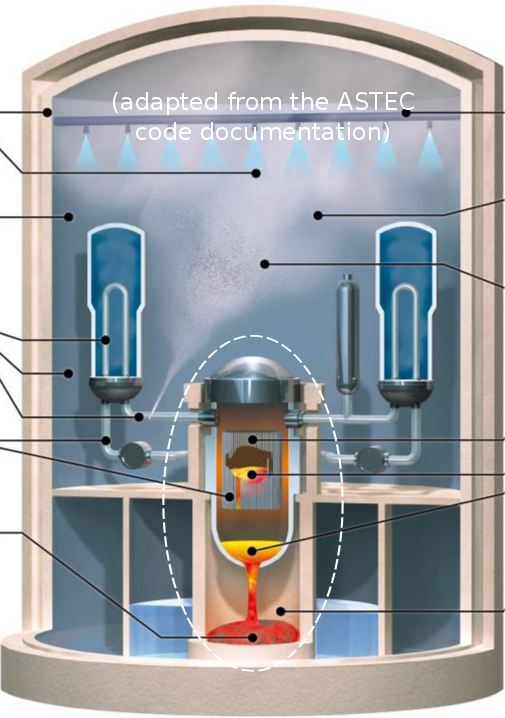
\includegraphics[width=\textwidth]{Figures/corium.png}
  \end{column}
  \end{columns}
  \item \emph{``Physique'' du corium} : ``mal connue'' 
  \begin{itemize}
    \item \emph{phénomènes} nombreux, pas forcément clairement identifiés ou \emph{``mal connus''} 
    \item des \emph{échelles temporelles et spatiales} pouvant très \emph{différentes}
  \end{itemize}
\end{itemize}
\end{frame}
\Titre{Dégradation en c\oe ur et progression de l'accident vers le fond de cuve}
\begin{frame}[fragile]
\begin{center}
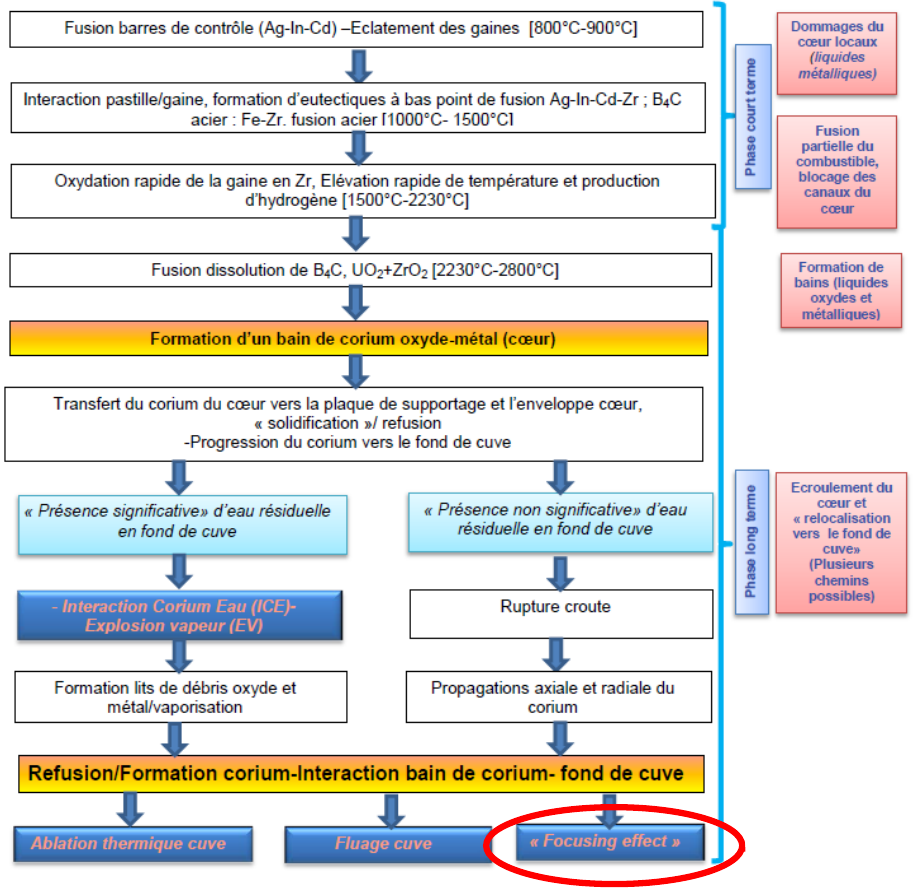
\includegraphics[height=\textheight]{Figures/transition_PP.png}
\end{center}
\end{frame}
\subsection{Ce $\mu$-projet: stratégie de rétention en cuve}
\Titre{Ce $\mu$-projet: stratégie de rétention en cuve}
\begin{frame}[fragile]
Rétention du corium en cuve ou ``In-Vessel Retention'' (IVR)
\begin{columns}
\begin{column}{0.7\textwidth}
\begin{itemize}
\item Quoi~? Une \emph{stratégie de gestion de l'accident de fusion du c\oe ur} introduite dans les années 1990 \cite{Henry1993,Tuomisto1994}
\item Pourquoi~? \emph{Garder l'intégrité de la cuve} pour y contenir les matériaux fondus du c\oe ur
\item Comment~? \emph{Dépressurisation précoce} de la cuve et \emph{renoyage précoce du puits de cuve} 
\end{itemize}
\end{column}
\begin{column}{0.3\textwidth}
\centering 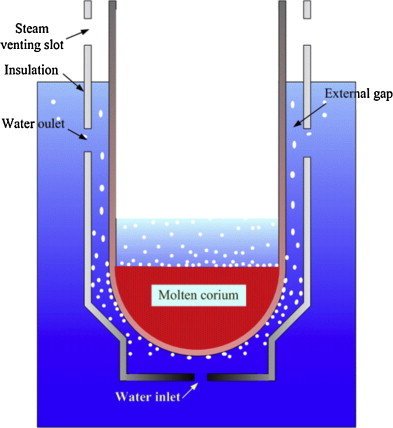
\includegraphics[height=0.5\textheight]{Figures/ivr.jpg}
\end{column}
\end{columns}
\begin{itemize}
\item Une mitigation réussie si :
\begin{itemize}
  \item le \emph{refroidissement de la cuve} par circulation d'eau est ``efficace'' de manière à éviter une ablation (locale) de la cuve sur toute son épaisseur \textit{i.e.} \\
  rester en \emph{régime d'ébullition nucléée} $\leftrightarrow$ éviter la crise d'ébullition (assèchement) $\leftrightarrow$ garantir que le \emph{flux de chaleur} en paroi externe de la cuve reste \emph{inférieur au flux critique}
  \item la cuve, partiellement ablatée, \emph{résiste mécaniquement} à la charge imposée (poids du bain et éventuels pics de pression) en transitoire et sur le long terme
\end{itemize}
\end{itemize}
\end{frame}
\begin{frame}[fragile]
\begin{columns}
\begin{column}{0.45\textwidth}
Trois sujets (interdépendants) pour une démonstration d'IVR:
\begin{itemize}
  \item \emph{comportement du corium en cuve} 
  \item \emph{thermohydraulique diphasique} de l'eau dans le \emph{puits de cuve}
  \item \emph{thermomécanique de la cuve}
\end{itemize}
\end{column}
\begin{column}{0.55\textwidth}
\begin{figure}[H]
\centering 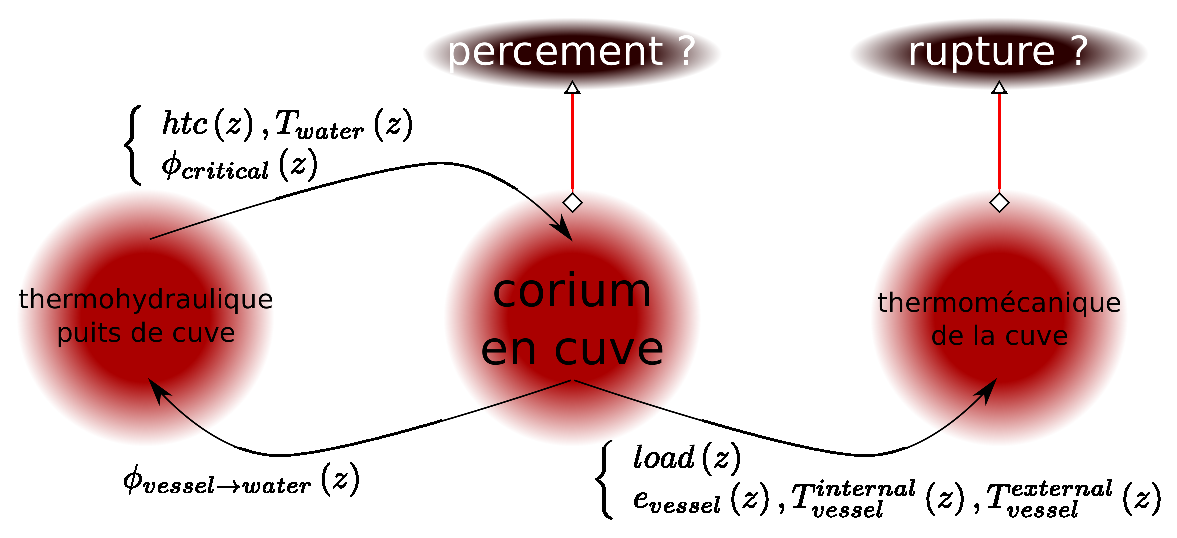
\includegraphics[width=1.0\textwidth]{Figures/ivr_topics.eps}
\caption{Vue schématique des thématiques associées à une démonstration d'IVR}
\end{figure}
\end{column}
\end{columns}
On se concentrera ici sur la question du \emph{comportement du corium en cuve}
\begin{itemize}
\item thermohydraulique multiphasique $\rightarrow$ chargement thermique sur la cuve
\item système ouvert $\leftarrow$ apport d'acier fondu par ablation de structures internes et de la paroi de la cuve
\end{itemize}
\end{frame}

%%%%%%%%
\section{Le corium en fond de cuve: version simple}
\Intercalaire{Le corium en fond de cuve: version simple}
\Titre{Le corium en fond de cuve: version simple}
\begin{frame}[fragile]
Evaluation \emph{stationnaire ``enveloppe''} des flux de chaleur transmis à la cuve
\begin{itemize}
\item approche ``historique'' utilisée en particulier dans la \emph{démonstration de sûreté} des réacteurs AP600 puis \emph{AP1000} \cite{Esmaili2004} 
\item dans sa version initiale, \emph{configuration ``à deux couches''} :
\begin{columns}[T]
    \begin{column}{0.35\textwidth}
      \begin{figure}[H]
\centering 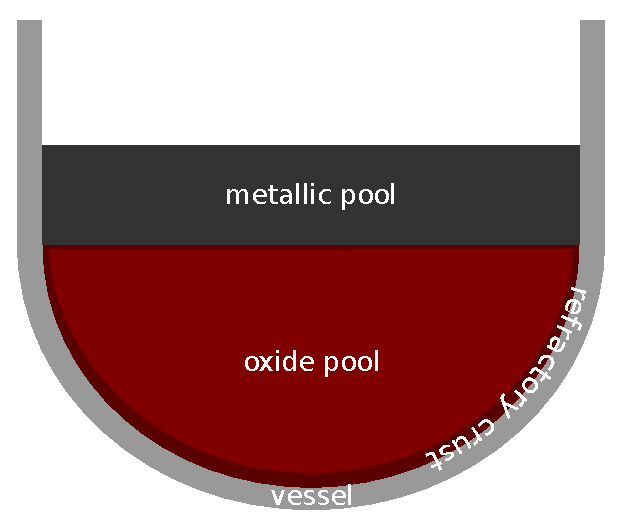
\includegraphics[height=0.4\textheight]{Figures/TD_2layer_2.eps}
\caption{Configuration à deux couches}
      \end{figure}
    \end{column}
    \begin{column}{0.65\textwidth}
    \begin{itemize}
    \item en bas : une \emph{phase oxyde} entourée d'une croûte réfractaire 
    \item en haut : une \emph{phase métallique} en contact direct avec la paroi de la cuve en fusion
    \item masses et compositions de ces deux couches obtenus à partir de simulations de la dégradation en c\oe ur et d'hypothèses simplistes sur la fusion des structures et de la paroi de la cuve
    \end{itemize}
    \end{column}
\end{columns}
  \item utilisée pour des \emph{études statistiques avec une modélisation intégrale} (\textit{cf.} TD à venir) : paramètres du modèle et définissant la configuration en fond de cuve ``probabilisés'' 
\end{itemize}

\end{frame}
\Titre{Corium en cuve et écoulements en convection naturelle}
\begin{frame}[fragile]
Deux configurations d'\emph{écoulements en convection naturelle} :
\begin{columns}[T]
    \begin{column}{0.3\textwidth}
\centering 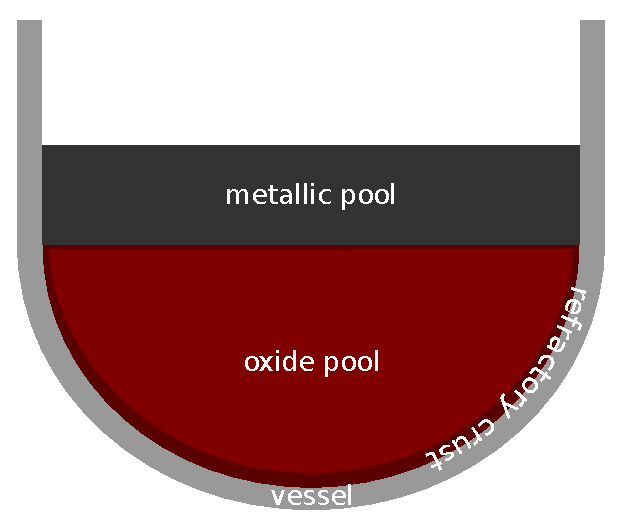
\includegraphics[height=0.3\textheight]{Figures/TD_2layer_2.eps}
    \end{column}
    \begin{column}{0.7\textwidth}
    \begin{itemize}
    \item couche métallique supérieure chauffée par le dessous, refroidie latéralement, par le dessus
    \item bain oxyde chauffé ``en volume'' et refroidie à sa frontière
    \end{itemize}
    \end{column}
\end{columns}
\vskip \baselineskip
\emph{Propriétés des liquides mis en jeu} et comparison à l'eau liquide 
\begin{tiny} \begin{center}
  \begin{tabularx}{0.9\textwidth}{|l|R|R|R|R|} \hline
  \multicolumn{1}{|c|}{\multirow{2}{*}{Propriété}} & \multicolumn{1}{c|}{\multirow{2}{*}{Unité}} & \multicolumn{2}{c|}{Valeur (\emph{ordre de grandeur})} & Valeur eau \n
  & & \multicolumn{1}{c|}{Oxyde} & \multicolumn{1}{c|}{Métal} & \multicolumn{1}{c|}{à 25$^o$C, 1bar} \n \hline
  masse volumique $\rho$ & kg.m$^{-3}$ & ~8000 & ~7000 & 997 \n
  conductivité thermique $\lambda$ & W.m$^{-1}$.K$^{-1}$ & 5 & 25 & 0.61\n
  \emph{viscosité cinématique} $\nu$ & m$^2$s.$^{-1}$ & 5$\times$10$^{-7}$ & 5$\times$10$^{-7}$ & 8.9$\times$10$^{-7}$ \n
  capacité calorifique massique $Cp$& J.K$^{-1}$.kg$^{-1}$ & 500 & 800 & 4182 \n
  coefficient de dilatation thermique isobare $\beta$ & K$^{-1}$ & 10$^{-4}$ & 10$^{-4}$ & 2.6$\times$10$^{-4}$\n \hline
  diffusivité thermique $\alpha=\frac{\lambda}{\rho Cp}$ & m$^2$s.$^{-1}$ & 10$^{-6}$ & 4$\times$10$^{-6}$ & 1.5$\times$10$^{-7}$ \n
  $\emph{Pr}=\frac{\nu}{\alpha}=\frac{\text{diffusivité de la quantité de mouvement}}{\text{diffusivité de la chaleur}}$ & - & 0.5 & 0.1 & 5.9 \n \hline
  \end{tabularx}
\end{center}
  \begin{remark}
  On considèrera que le corium en cuve peut être traité comme un fluide Newtonien (dans la gamme de température/composition d'intérêt); \danger $\ne$ pour le corium ``hors-cuve''
  \end{remark}
\end{tiny} 
\end{frame}

%%%%%%%%
\subsection{Thermohydraulique de la couche métallique supérieure}
\Titre{Thermohydraulique de la couche métallique supérieure}
\begin{frame}[fragile]
\begin{columns}[T]
    \begin{column}{0.3\textwidth}
\vskip -\baselineskip
\centering 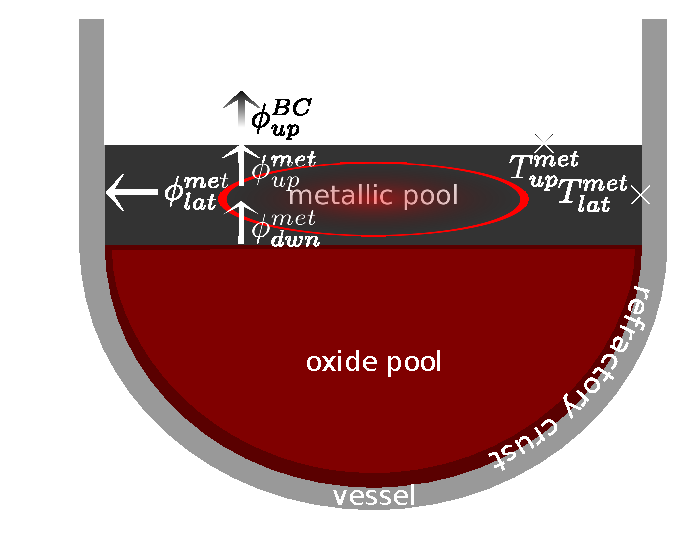
\includegraphics[height=0.4\textheight]{Figures/TD_2layer_metal.eps}
    \end{column}
    \begin{column}{0.7\textwidth}  
    \begin{scriptsize}
    \begin{itemize}
    \item en bas (croûte) : \textit{sans glissement}, $\phi^{met}_{dwn}$ imposé
    \item latéralement (cuve) : {\scriptsize $\left\{\begin{array}{l} \text{sans glissement} \\ T^{met}_{lat} \text{ imposée (fusion) / } \phi^{met}_{lat}=\phi^{vessel}_{lat} \end{array}\right.$}
    \item en haut : {\scriptsize $\left\{\begin{array}{l} \text{sans glissement / surface libre} \\ \text{température imposée} T^{met}_{up} \text{ / } \phi^{met}_{up}=\phi^{met}_{BC} \end{array}\right.$}
    \end{itemize} 
    \end{scriptsize}
    \end{column}
\end{columns}
\begin{itemize}
\item Sous l'\emph{hypothèse de Boussinesq}, équations de conservation locales :
\begin{columns}[T]
    \begin{column}{0.58\textwidth}
\begin{scriptsize}
\vskip -\baselineskip
\begin{eqnarray*}
\div{\vec{v}} &=& 0 \\
\frac{\partial \vec{v}}{\partial t} + \vec{v} \cdot \grad{\vec{v}} &=& -\frac{1}{\rho_0}\grad{p} + \nu_0 \Lapl{\vec{v}} - \vec{g} \beta_0 \left(T-T_0\right) \\
\frac{\partial T}{\partial t} + \vec{v} \cdot \grad{T} &=& \alpha_0 \Lapl{T}
\end{eqnarray*}
\vskip -\baselineskip
\end{scriptsize}
    \end{column}
    \begin{column}{0.42\textwidth}
\begin{scriptsize}
    Bilan thermique intégral :
    \begin{equation*} mCp \frac{d\bar{T}}{dt} = \phi^{met}_{dwn} S^{met}_{dwn} - \phi^{met}_{lat} S^{met}_{lat} - \phi^{met}_{up} S^{met}_{up} \end{equation*}
\end{scriptsize}
    \end{column}
% \vskip -\baselineskip
\end{columns}
\item Les \emph{``paramètres de contrôle''} sont :
\begin{itemize}
\item $Pr$, $Gr=\frac{g\beta\Delta T H^3}{\nu^2}=\frac{\text{forces de gravité}}{\text{forces visqueuses}}$ (ou $Ra=Gr \cdot Pr$)
\item le rapport d'aspect $\frac{H}{R}$ (cylindre de rayon $R$, hauteur $H$)
\item éventuellement d'autres selon les conditions en limite supérieure
\end{itemize}
\item Les `\emph{`quantités d'intérêt''} sont $Nu_{lat}$ et $Nu_{up}$ ($Nu=\frac{\text{flux de chaleur convectif}}{\text{flux de chaleur conductif}}=\frac{htc \times L}{\lambda}$ )
\end{itemize}
\end{frame}
\begin{frame}[fragile]
\begin{itemize}
\item De première importance car possibilité de \emph{concentration de flux (``focusing effect'')} \\ \textit{i.e.} $\frac{\phi^{met}_{lat}}{\phi^{met}_{dwn}}>1$ $\rightarrow$ \emph{risque principal de percement ``thermique'' de la cuve}
\item Configuration étudiée expérimentalement e.g. dans la \emph{campagne BALI-Metal} (CEA Grenoble) : avec de l'eau (\danger $Pr$), en géométrie parallépipédique $\rightarrow$ $\frac{\phi^{met}_{lat}}{\phi^{met}_{dwn}}\left(H\right)$
\item Schéma grossier de l'écoulement (Figure tirée de \cite{Villermaux1999})
\begin{columns}[T]
    \begin{column}{0.6\textwidth}
\centering 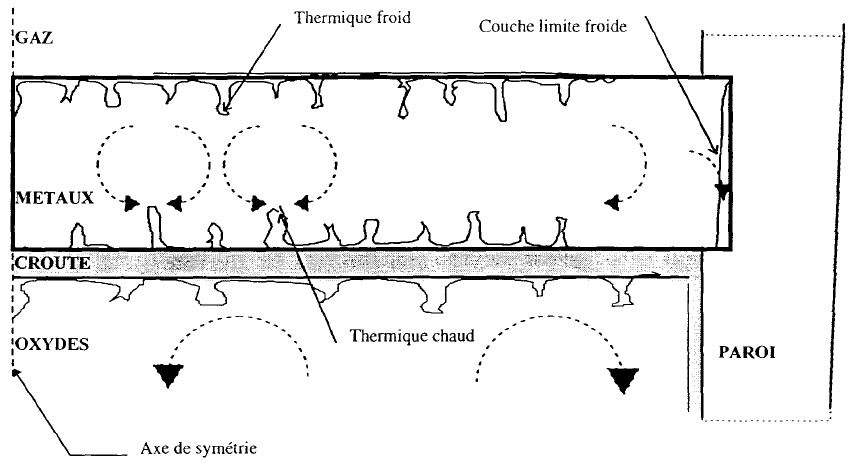
\includegraphics[width=0.8\textwidth]{Figures/metal_layer_flow.png}
    \end{column}
    \begin{column}{0.5\textwidth}
    \hskip -1cm \begin{minipage}{\textwidth}
    \begin{itemize}
    \item couche de fluide plus chaud en haut\\ $\rightarrow$ panaches (``thermiques'') chauds intermittents
    \item couche de fluide plus froid en haut \\ $\rightarrow$ panaches froids intermittents
    \item couche limite froide latérale \\ $\rightarrow$ accélération locale
    \end{itemize}
    \end{minipage}
    \end{column}
\end{columns}
\item Transition d'un écoulement laminaire à turbulent ``a partir'' de $H \sim10$cm
\item \emph{En première approche}, écoulement appréhendé comme la \emph{``juxtaposition''} de cellules de \emph{convection Rayleigh-Bénard} et d'une \emph{recirculation à la frontière latérale}
\end{itemize}
\end{frame}
\subsubsection{Conditions thermiques en limites axiales : instabilité de Rayleigh-Bénard}
\Titre{Couche métallique supérieure - instabilité de Rayleigh-Bénard}
\begin{frame}[fragile]
\begin{itemize}
\item Ecoulement \emph{conditionnellement instable} $Ra>Ra_c$ et transition \emph{laminaire - turbulent} (``douce'' puis ``dure'' puis ``asymptotique'')
\begin{minipage}{0.9\textwidth}
\begin{tabular}{cc}
\tiny{(Figures tirées de \cite{Gauthier2008})} & \multirow{2}{*}{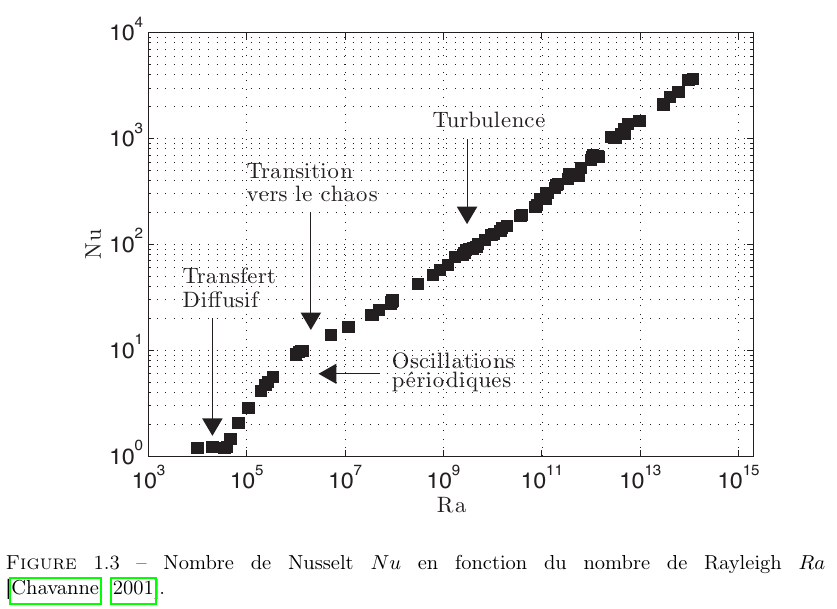
\includegraphics[width=0.5\textwidth]{Figures/Fig1_3_Gauthier2008.png}} \\
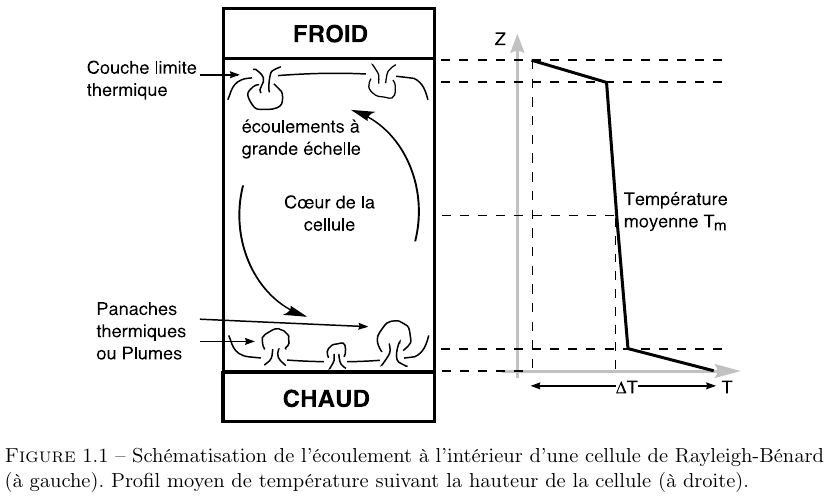
\includegraphics[width=0.5\textwidth]{Figures/Fig1_1_Gauthier2008.png} & \\
\end{tabular}
\end{minipage}
\vskip \baselineskip 
\item turbulence ``douce'' ($Ra_t<Ra<10^7$) : hypothèse de Markus (couches limites haute et basse indépendantes) $\rightarrow$ épaisseur $\delta = \frac{H}{2 Nu}$ indépendante de $H$ $\rightarrow$ $Nu \propto Ra^{\frac{1}{3}}$
\item au-delà, turbulence ``dure'' $\rightarrow$ $Nu \propto Ra^{\frac{2}{7}}$ ; asymptotique $\rightarrow$ $Nu \propto Ra^{\frac{1}{2}}$
\end{itemize}
\begin{tiny}
\begin{remark}[H. Bénard (1900)]
``Je n’ai pas la prétention d’avoir épuisé un sujet aussi nouveau : bien des points restent à éclaircir, même sans sortir du point de vue expérimental ; mais je serais heureux si mon travail, tout incomplet qu’il est, contribuait à attirer l’attention des expérimentateurs sur les domaines inexplorés de la Physique moléculaire et de la Mécanique des fluides''
\end{remark}
\end{tiny}
\vskip -0.5\baselineskip 
\scriptsize $\rightarrow$ Un v\oe u exaucé ! Toujours \emph{un sujet ``intense'' de recherche} (simulation numérique et expérience)
\end{frame}
\subsubsection{Conditions thermiques en limite latérale : refroidissement}
\Titre{Couche métallique supérieure - refroidissement latéral}
\begin{frame}[fragile]
\begin{itemize}
\item Ecoulement \emph{inconditionnellement instable} \begin{minipage}{0.05\textwidth}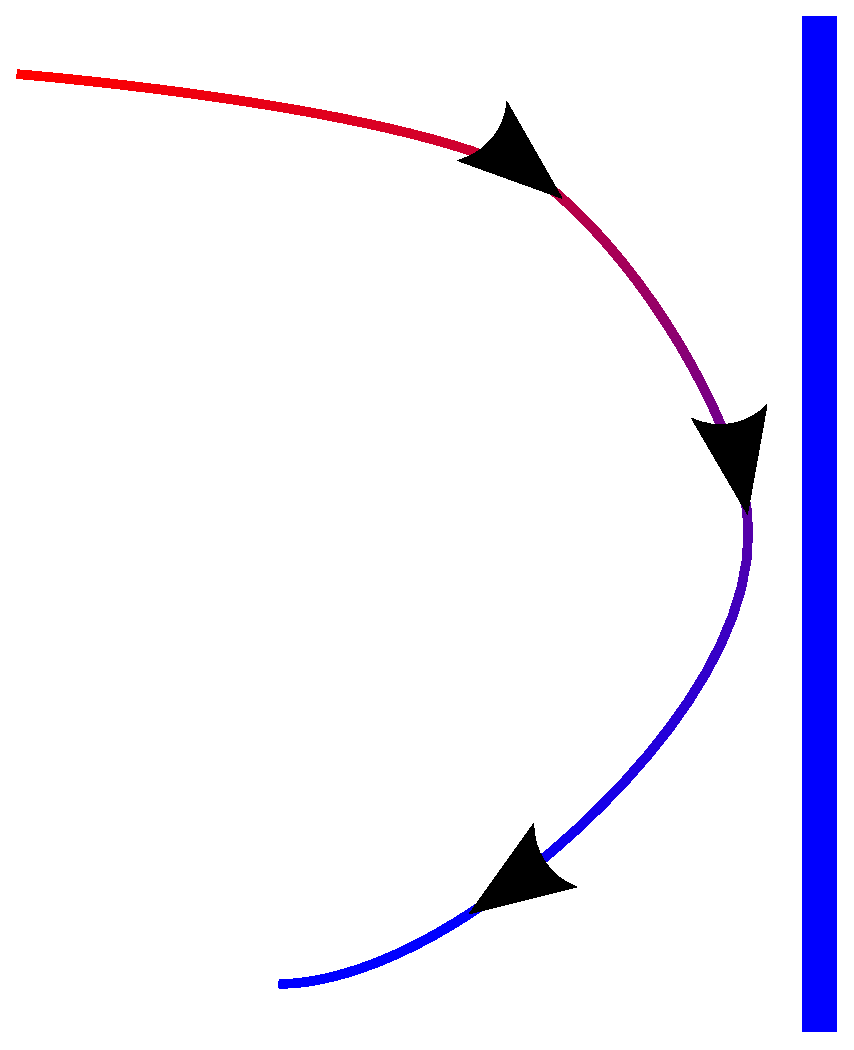
\includegraphics[width=\textwidth]{Figures/vertical_plate.eps} \end{minipage}
\item \emph{Impact sur le profil de température} pour $Pr$ faible {\tiny (Figure tirée de \cite{Tran2013})} \\
\begin{center} \vskip -\baselineskip ~ \\ 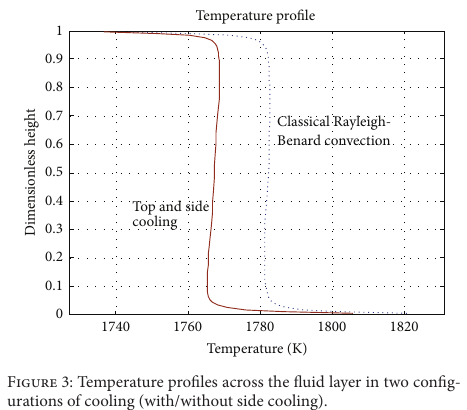
\includegraphics[width=0.4\textwidth]{Figures/Fig3_Tran2013.png} \end{center}
\item Malgré (à cause ?) de la complexité pour cette couche métallique, les \emph{modèles intégraux} ou ``grossièrement maillés'' ont recours à des \emph{corrélations} établies séparément pour des \emph{configurations ``unidimensionnelles''} $\rightarrow$ \textit{cf.} TD
\item Avec des limites (et des perspectives) que nous aborderons en 2$^{\text{ème}}$ partie de cours
\end{itemize}
\end{frame}

%%%%%%%%
\subsection{Thermohydraulique du bain oxyde}
\subsubsection{Solidification à l'interface}
\Titre{Bain oxyde - solidification à l'interface}
\begin{frame}[fragile]
\begin{columns}[T]
    \begin{column}{0.25\textwidth}
\centering 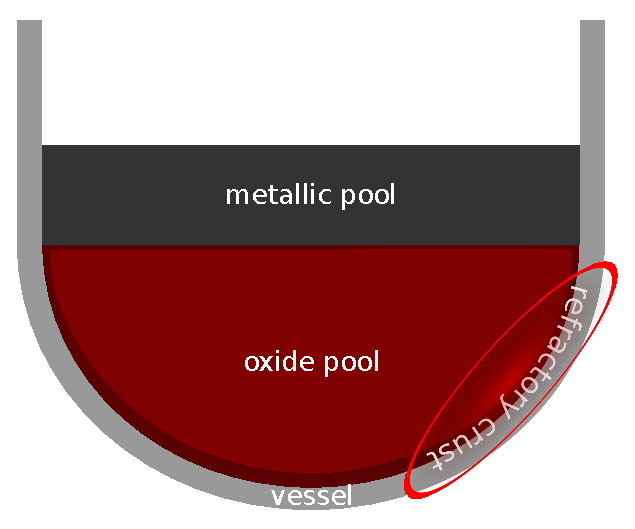
\includegraphics[height=0.3\textheight]{Figures/TD_2layer_crust.eps}
    \end{column}
    \begin{column}{0.75\textwidth}
\begin{itemize}
\item Corium oxyde : \emph{système ternaire} $\left(U_y,Zr_{1-y}\right)O_{2-x}$ ``en manque d'oxygène'' ($x\ge0$)
\item Température de liquidus $T_{liq}^{oxyde} \in [2300, 2950]$K suivant $y$ et $x$, toujours supérieur à $T_{liq}^{acier} \sim 1600$K $\rightarrow$ \emph{solidification à l'interface bain oxyde/cuve}
    \end{itemize}
    \end{column}
\end{columns}
\begin{minipage}{0.8\textwidth}
\begin{tabular}{cc}
\tiny{Figures tirées de \cite{Quaini2015} (échantillon $O_{0.39}U_{0.103}Zr_{0.507}$}) & \multirow{2}{*}{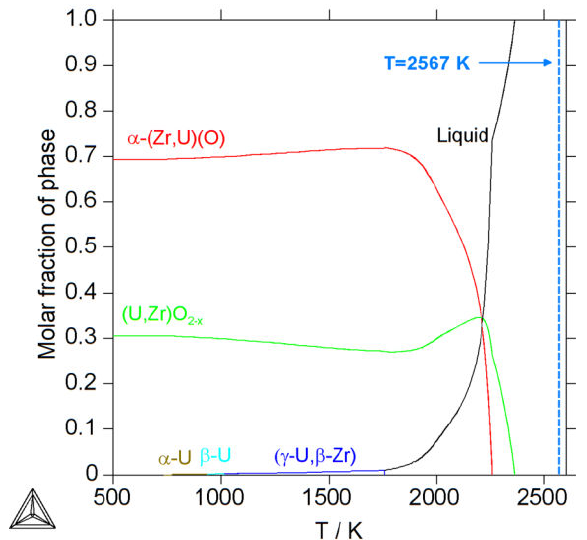
\includegraphics[width=0.42\textwidth]{Figures/Fig18a_Quaini2015.png}} \\
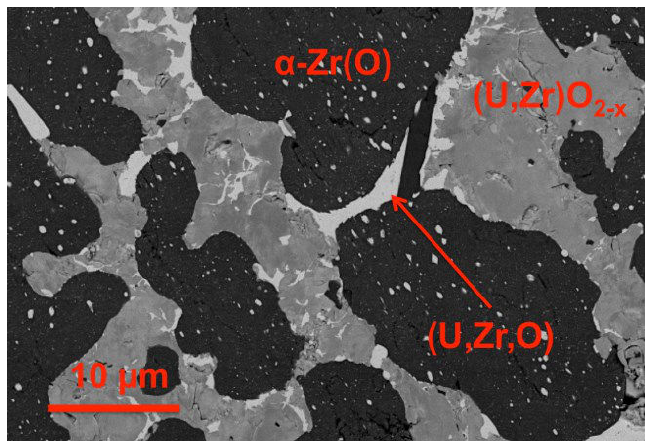
\includegraphics[width=0.5\textwidth]{Figures/Fig18b_Quaini2015.png} & \\
\tiny{microstructure observé} & \tiny{chemin de solidification (``lever-rule'') calculé}
\end{tabular}
\end{minipage}
\begin{itemize}
\item Solidification d'un \emph{matériau multicomposant} potentiellement \emph{compliquée} ... 
\end{itemize}
\end{frame}
\begin{frame}[fragile]
\begin{itemize}
\item ... corium $\left(U_y,Zr_{1-y}\right)O_{2-x}$ : le plus souvent, les \emph{hypothèses simplificatrices} suivantes :
\begin{itemize}
  \item un \emph{front de solidification à l'équilibre thermodynamique} $\rightarrow$ phase solide formée associée $\left(U_{y'},Zr_{1-y'}\right)O_{2-x'}$ à la température de liquidus du liquide à l'interface 
  \item \emph{variations de composition négligées} (liquide homogène et $x'=x$, $y'=y$)
\end{itemize}
\item Ainsi, \emph{comme pour un ``corps pur''}, solidification à l'interface régit par le déplacement d'un \emph{front plan} (\emph{condition de Stefan}, cas particulier du thèorème de Kotchine)
\begin{itemize}
  \item température imposée à l'interface $T^{\textrm{ls}}=T_{liq}^{oxyde}$
  \item condition de saut sur les flux à l'interface liquide/solide $\textrm{ls}$ : 
\begin{columns}
\begin{scriptsize}
\begin{column}{0.55\textwidth}
\begin{eqnarray*}
  \vec{v}^{\textrm{ls}}(\vec{r}, t) &=& \frac{\vec{n}^{\textrm{ls}}}{\rho_l \Delta h_{ls}} \left(-\lambda_l \grad{T_l}(\vec{r}, t) + \lambda_s \grad{T_l}(\vec{r}, t) \right) \cdot \vec{n}^{\textrm{ls}} \\
  &&\text{(vitesse locale)}\\
  \frac{dm^{\textrm{ls}}(t)}{dt} &=& \frac{1}{\Delta h_{ls}} \left(\phi_l^{\textrm{ls}}(t) - \phi_s^{\textrm{ls}}(t)\right) S^{\textrm{ls}} \\
  && \text{(débit massique intégral)}
\end{eqnarray*}
\end{column}
\begin{column}{0.45\textwidth}
\begin{itemize}
\item $\vec{n}^{\textrm{ls}}$ : normal orientée du liquide vers le solide
\item $\Delta h_{ls}$ : chaleur latente spécifique de solidification
\end{itemize}
\end{column}
\end{scriptsize}
\end{columns}
\end{itemize}
\item En géométrie \emph{1D plan}, en  \emph{régime stationnaire}, épaisseur du solide (sans dissipation interne de puissance) donnée par \emph{$e_{s} = \lambda_{s}\times \frac{\text{différence de température d'un bord à l'autre}}{\text{flux de chaleur}}$}
\end{itemize}
\end{frame}
\subsubsection{Convection naturelle par chauffage volumique}
\Titre{Bain oxyde - convection naturelle par chauffage volumique}
\begin{frame}[fragile]
\begin{columns}[T]
    \begin{column}{0.25\textwidth}
\centering 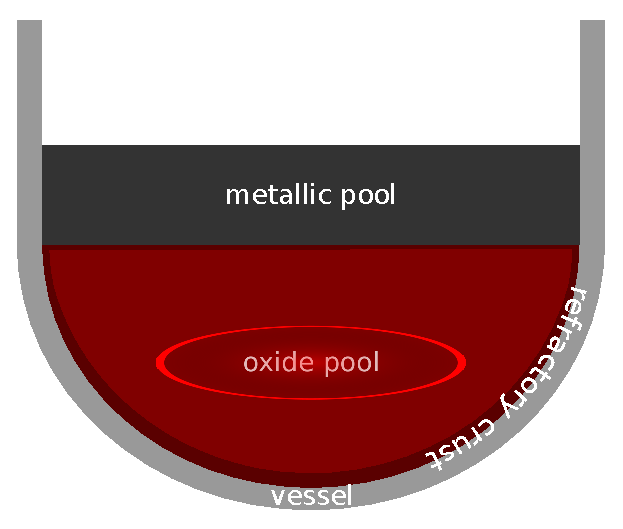
\includegraphics[height=0.3\textheight]{Figures/TD_2layer_oxide.eps}
    \end{column}
    \begin{column}{0.75\textwidth}
\begin{itemize}
    \item \emph{chauffage ``en volume''} (puissance résiduelle associée à la décroissance des produits de fission) : puissance volumique $q^{ox}$ (W/m$^3$)
    \item refroidissement en surfaces latérale et haute
    \item en \emph{régime turbulent} : $Ra_i^{ox}=\frac{g\left(H^{ox}\right)^5q^{ox}\beta^{ox}}{\lambda^{ox}\nu^{ox}\alpha^{ox}} \in [10^{14}, 10^{18}]$
    \end{itemize}
    \end{column}
\end{columns}
\begin{itemize}
\item Schéma de l'écoulement (Figure tirée de \cite{Bonnet1999})
\begin{columns}[T]
    \begin{column}{0.6\textwidth}
\centering 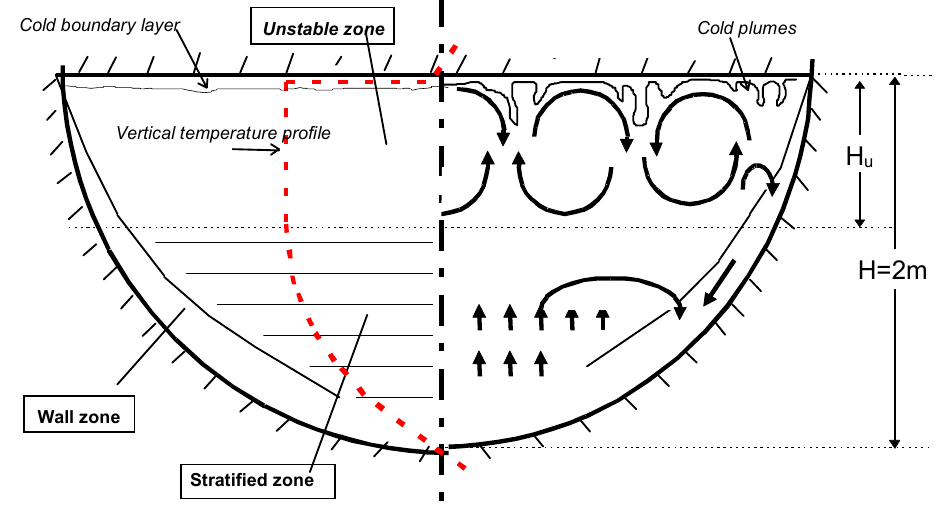
\includegraphics[width=0.8\textwidth]{Figures/Fig2_Bonnet2001.png}
    \end{column}
    \begin{column}{0.5\textwidth}
    \hskip -1cm \begin{minipage}{\textwidth}
    \begin{itemize}
    \item panaches froids et boucles de convection en haut
    \item couche limite froide latérale
    \item zone stratifiée thermiquement en bas
    \end{itemize}
    \end{minipage}
    \end{column}
\end{columns}
\end{itemize}
\end{frame}
\begin{frame}[fragile]
\begin{itemize}
\item En première approche, pour l'\emph{échange vers le haut}, parallèle entre cette \emph{configuration de ``Kulacki-Emara''} et une \emph{cavité de Rayleigh-Bénard} de hauteur $H_u$
\begin{columns}[T]
    \begin{column}{0.25\textwidth}
\centering 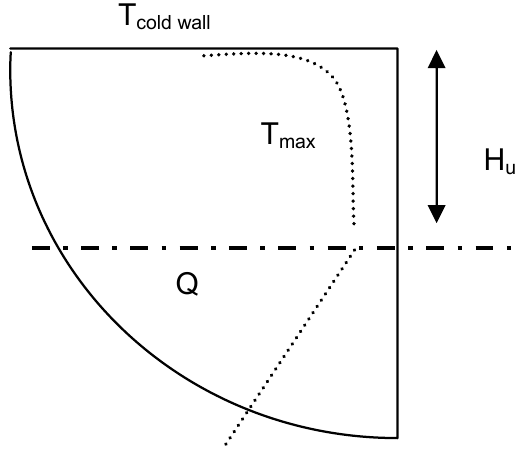
\includegraphics[width=1.0\textwidth]{Figures/p11_1_Bonnet2001.png}
    \end{column}
    \begin{column}{0.5\textwidth}
\centering 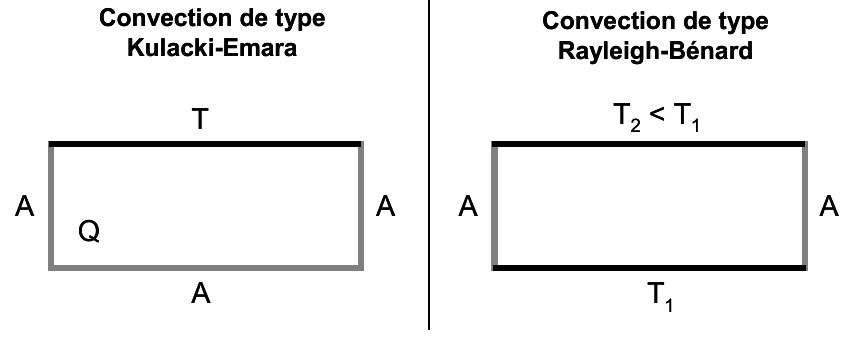
\includegraphics[width=1.0\textwidth]{Figures/KE_RB.png}
    \end{column}
    \begin{column}{0.25\textwidth}
\centering 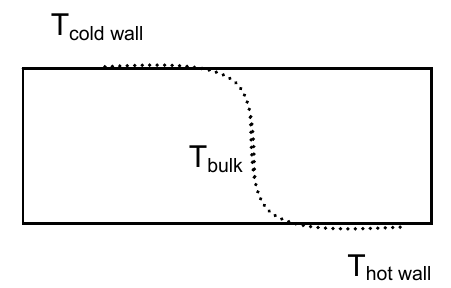
\includegraphics[width=1.0\textwidth]{Figures/p11_2_Bonnet2001.png} 
    \end{column}
\end{columns}
\begin{itemize}
  \item avec un nombre de Rayleigh exprimé en fonction de $\Delta T = \left(T_{max}-T_{cold\, wall}\right)$ et $H_u$
  \item à l'état stationnaire : $S_{up} \times \left(\frac{\lambda Nu_{up}}{H_u}\right) \Delta T = V \times q$
  \item ainsi, on peut travailler en nombre de \emph{Rayleigh interne} $Ra_i=\frac{g\left(H_u\right)^5\emph{q}\beta}{\lambda\nu\alpha}$ : \\
  $Nu^{RB}_{up} = a \times Ra^b Pr^c \Longleftrightarrow Nu^{KE}_{up} = 2a^{\frac{1}{b+1}} \times Ra_i^{\frac{b}{b+1}} Pr^{\frac{c}{b+1}}$
\end{itemize}
\item Pour l'\emph{échange latéral} (surface sphéro\"{\i}de), la \emph{transposition est moins évidente} ...
\end{itemize}
\end{frame}
\begin{frame}[fragile]
\begin{itemize}
\item ... de nombreuses \emph{expériences} ont été menées sur des  \emph{``géometries fond de cuve''} à échelle réduite avec différents matériaux simulants
\begin{columns}[T]
    \begin{column}{0.72\textwidth}
      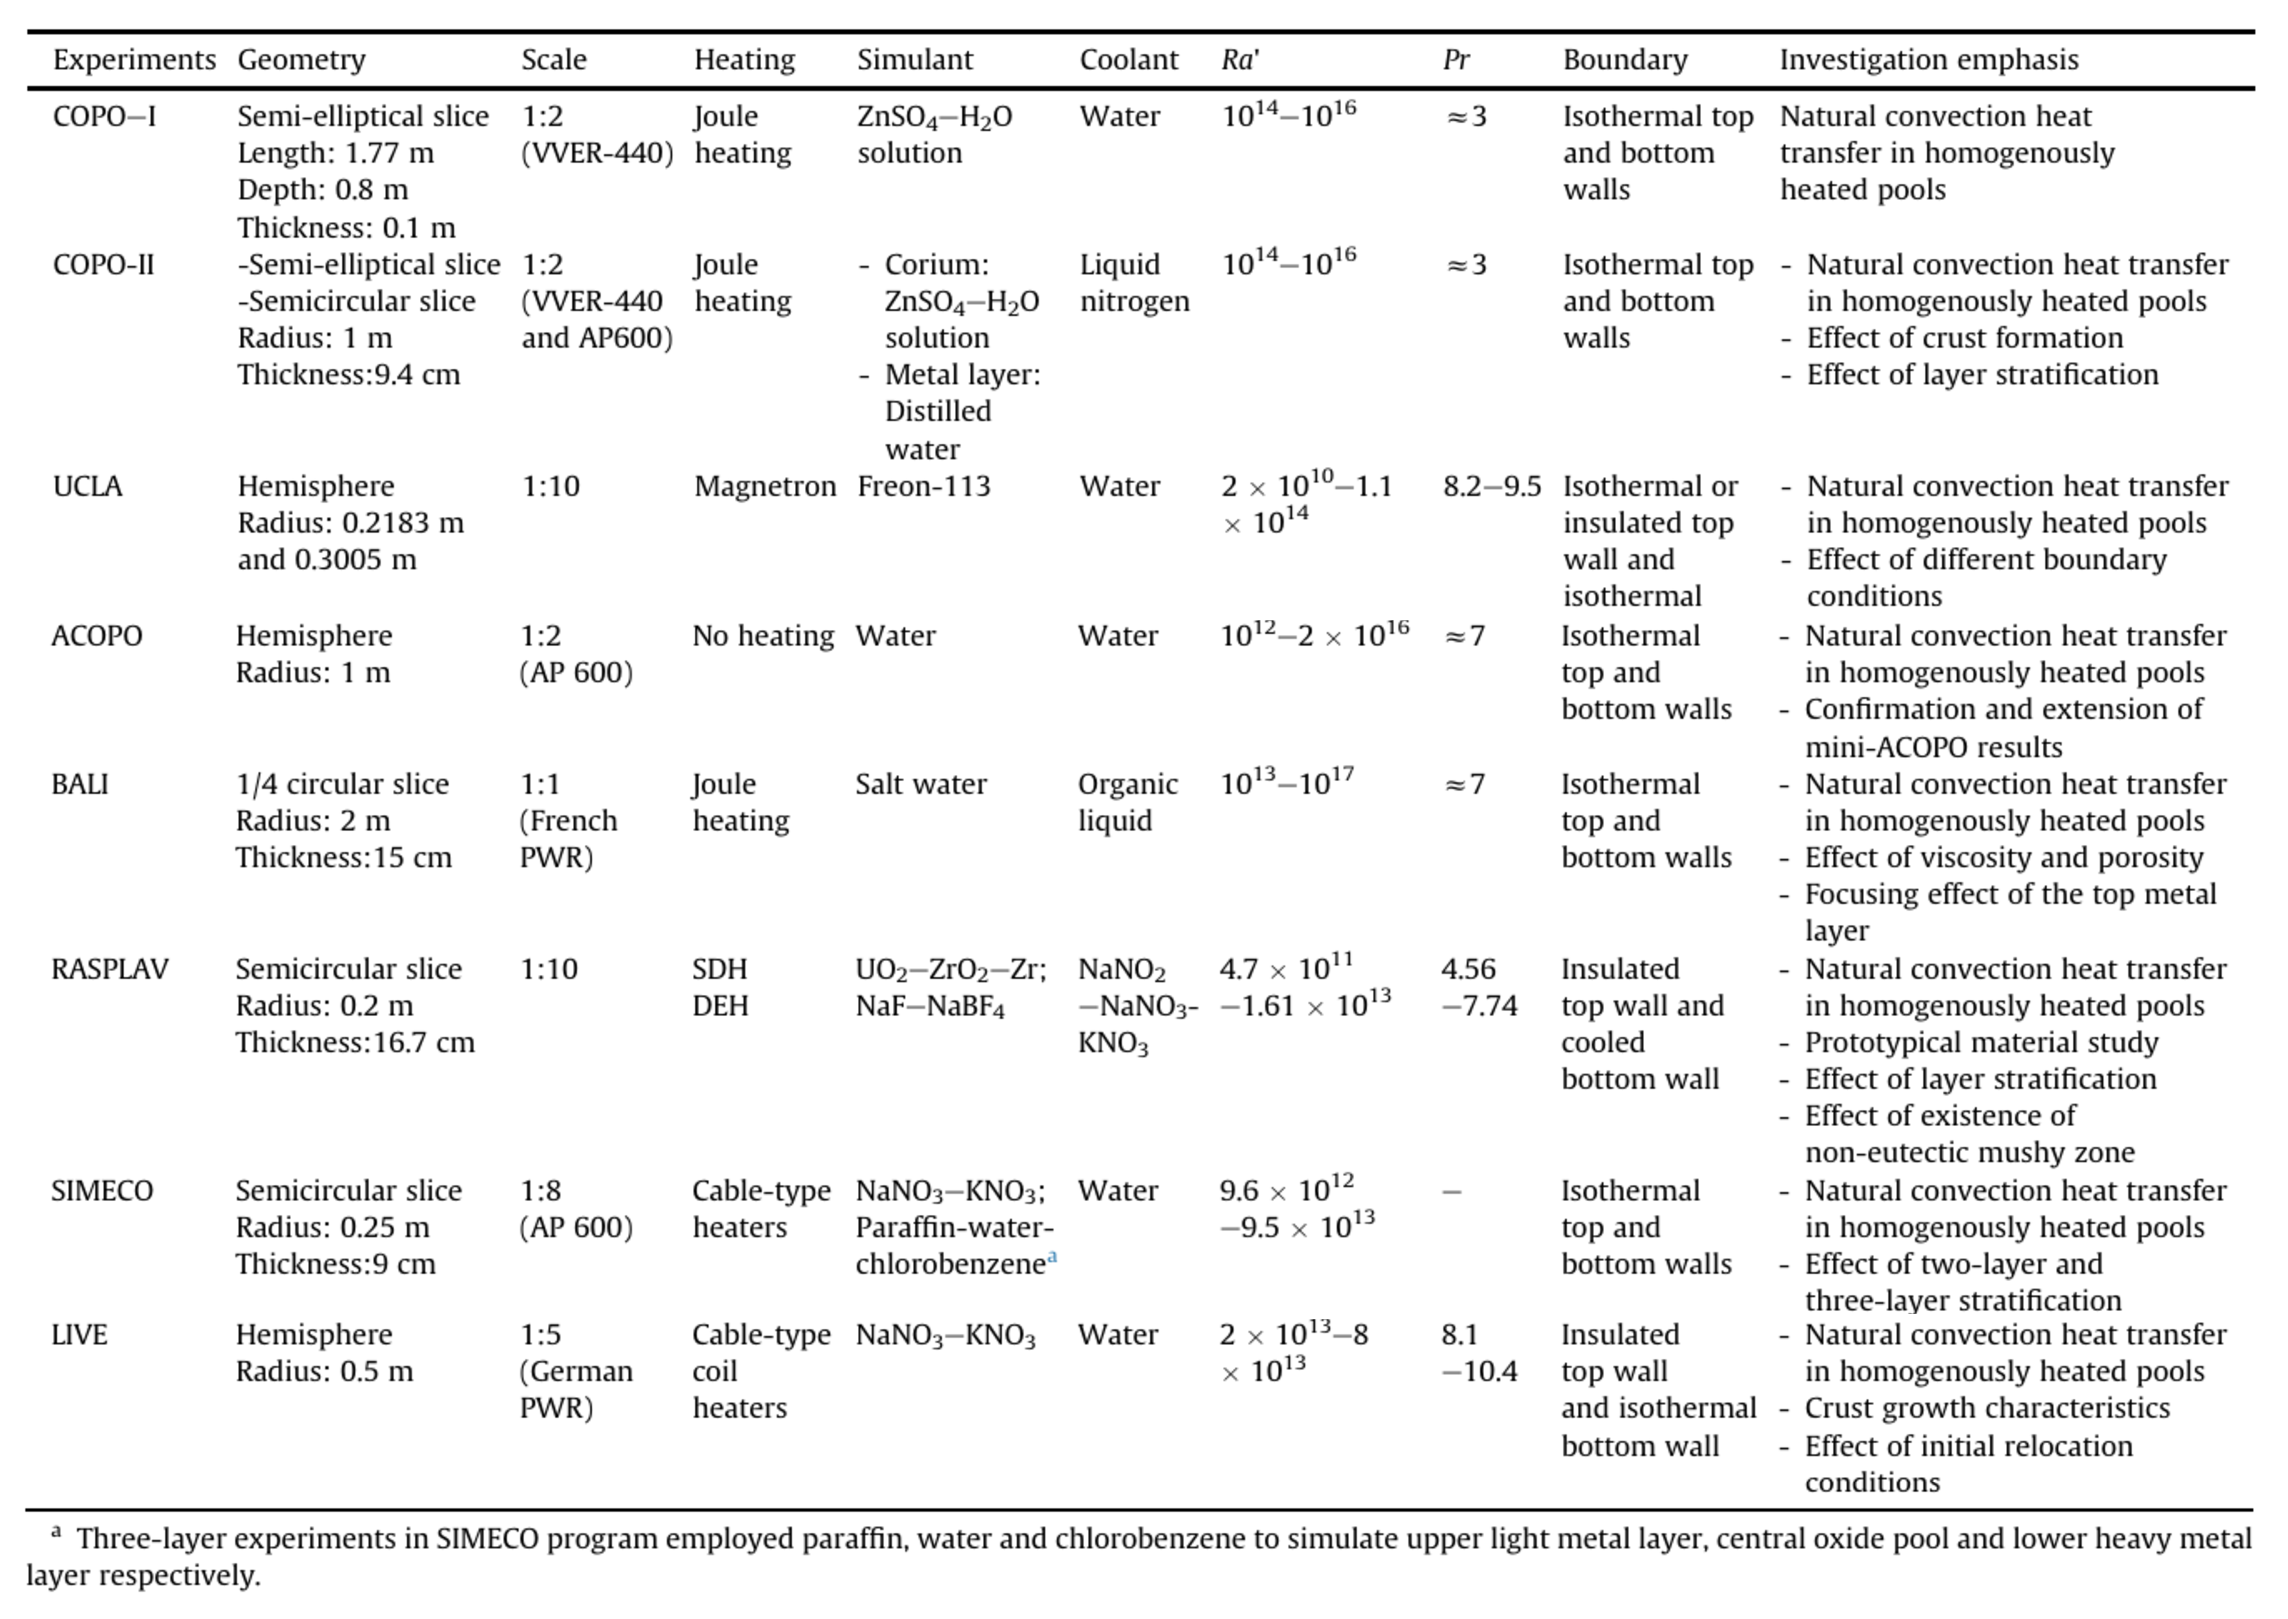
\includegraphics[height=0.8\textheight]{Figures/Tab3_Zhang2015.eps} \\
      {\tiny extrait d'un tableau de \cite{Zhang2015}}
    \end{column}
    \begin{column}{0.28\textwidth}
    \vskip -\baselineskip
    \centering
{\tiny BALI} \\ 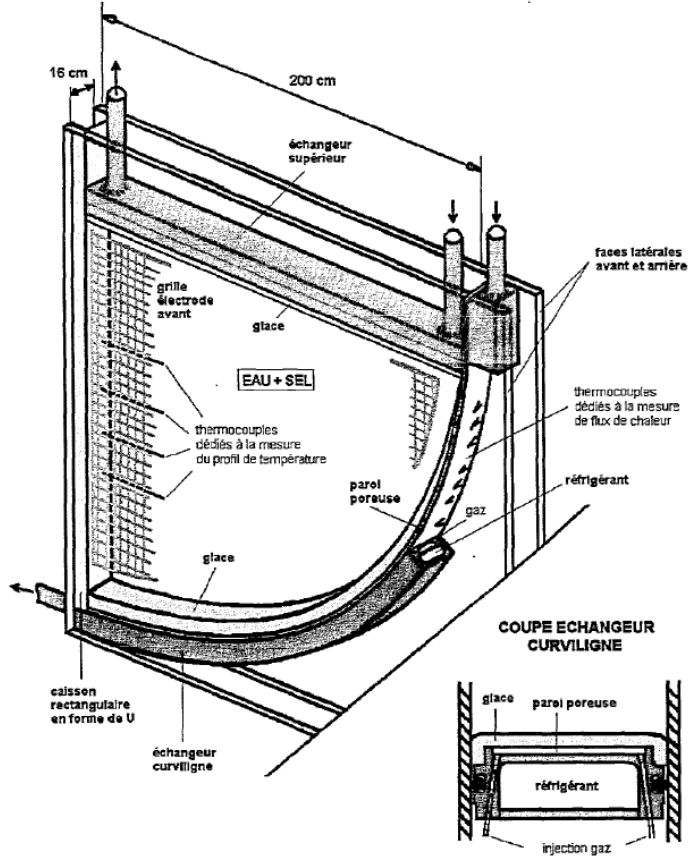
\includegraphics[width=1.0\textwidth]{Figures/bali.png} \\ 
{\tiny LIVE} \\ 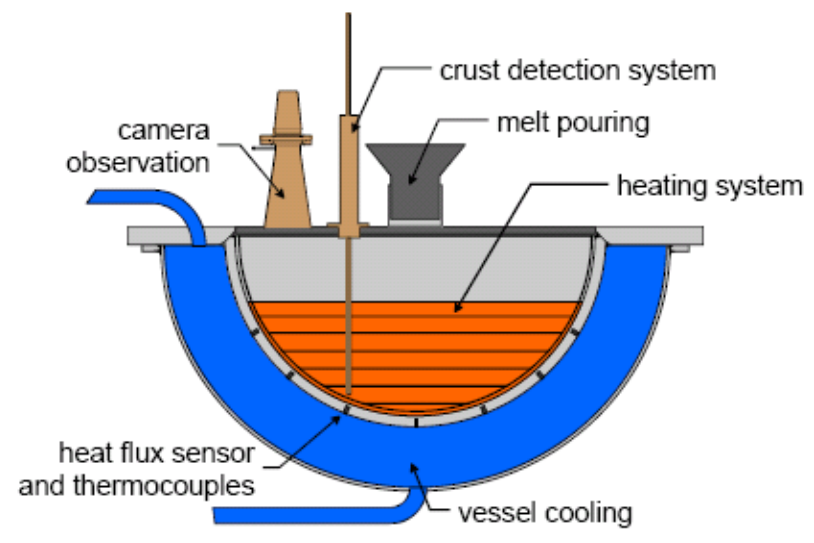
\includegraphics[width=1.0\textwidth]{Figures/live_1.png}
% 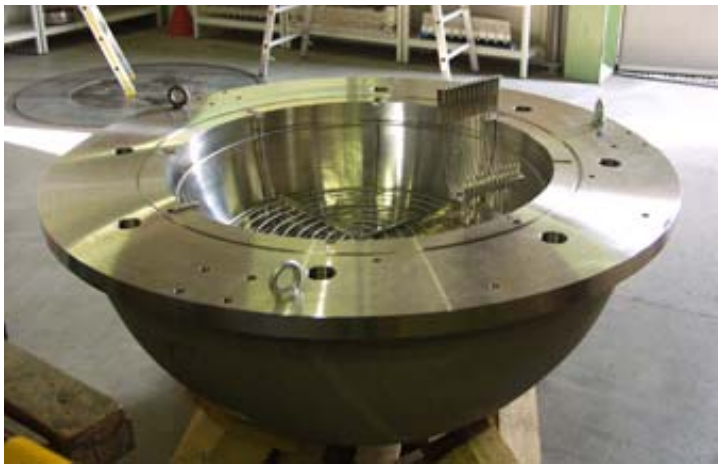
\includegraphics[width=1.0\textwidth]{Figures/live_2.png}
    \end{column}
\end{columns}
\end{itemize}
\end{frame}
\begin{frame}[fragile]
\begin{itemize}
\item Qui fournissent des \emph{corrélations} pour fermer les bilans des \emph{modèles intégraux}
\item Une \emph{dispersion des résultats qui augmente avec $Ra_i$} \danger
\begin{columns}[T]
    \begin{column}{0.4\textwidth}
\centering 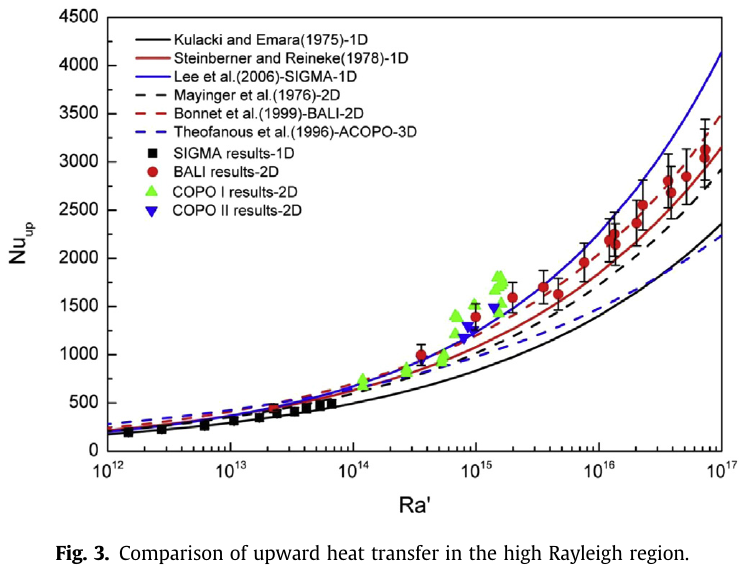
\includegraphics[width=1.0\textwidth]{Figures/Fig3_Zhang2015.png}
    \end{column}
    \begin{column}{0.4\textwidth}
\centering 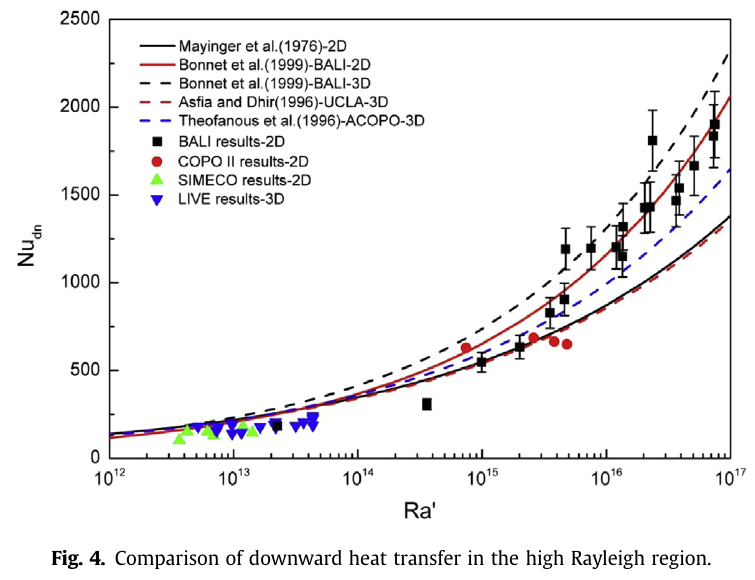
\includegraphics[width=1.0\textwidth]{Figures/Fig4_Zhang2015.png}
    \end{column}
\end{columns}
{\tiny (Figures tirées de \cite{Zhang2015})}
% \item ... mais pas une source majeure d'incertitude pour l'évaluation de l'IVR
\end{itemize}
\vskip -\baselineskip
\begin{columns}[T]
    \begin{column}{0.4\textwidth}
\begin{itemize}
\item Intérêt grandissant pour des simulations ``Computational Fluid Dynamics'' CFD
\end{itemize}
    \end{column}
    \begin{column}{0.6\textwidth}
\vskip -0.5\baselineskip
\centering 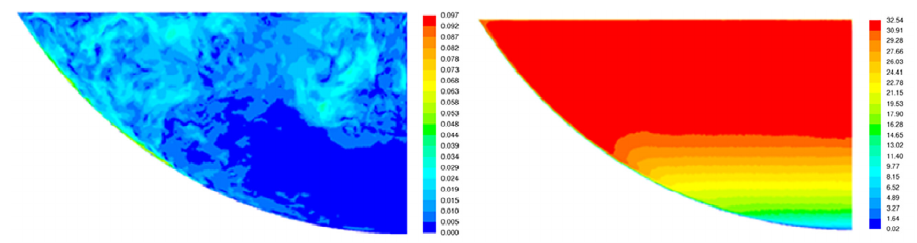
\includegraphics[width=1.0\textwidth]{Figures/Fig10a_Shams2019.png} \\ 
\vskip -0.5\baselineskip
{\tiny vitesse et température - calcul CFD-LES - essai BALI 1-15}
    \end{column}
\end{columns}
\vskip -\baselineskip
\centering {\tiny (Figure extraite de \cite{Shams2020})}
\end{frame}
%%%%%%%%
\subsection{TD : évaluation du bilan thermique intégral}
\Intercalaire{TD : évaluation du bilan thermique intégral}
\Titre{TD : évaluation du bilan thermique intégral}
\begin{frame}[fragile]
\begin{columns}[T]
    \begin{column}{0.4\textwidth}
      \begin{figure}[H]
\centering 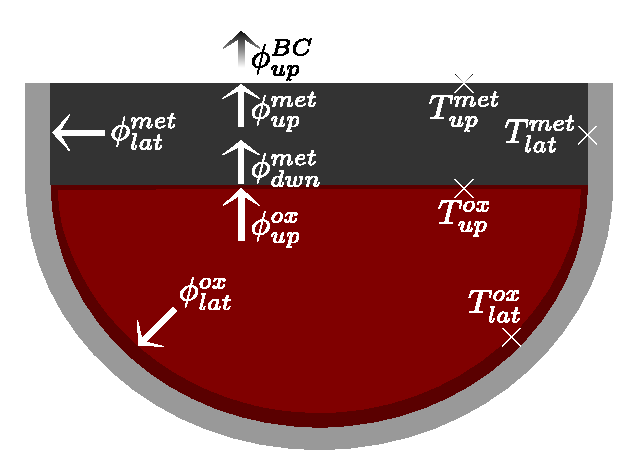
\includegraphics[height=0.4\textheight]{Figures/TD_2layer.eps}
\caption{Configuration à deux couches et notations des flux et températures}
      \end{figure}
    \end{column}
    \begin{column}{0.6\textwidth}
    \begin{itemize}
    \item Objectif: évaluation de la \emph{répartition de la puissance et du flux de chaleur} aux interfaces d'un bain de corium
    \item \emph{Configuration stationnaire à deux couches} :
    \begin{itemize} 
    \item en bas : une phase oxyde qui porte toute la puissance résiduelle entourée d'une croûte réfractaire 
    \item en haut : de l'acier liquide en contact direct avec la paroi de la cuve en fusion
    \end{itemize}
    \item Hypothèses et fermetures classiquement utilisées dans les codes de calculs (et que l'on vient de présenter pour la plupart)
    \end{itemize}
    \end{column}
\end{columns}
\vskip \baselineskip
\textit{cf.} description TD et notebooks Jupyter \\ {\scriptsize (\href{https://mybinder.org/v2/gh/niamorelreillet/INSTN-GA-micro-projet.git/master?filepath=TD?urlpath=lab}{https://mybinder.org/v2/gh/niamorelreillet/INSTN-GA-micro-projet.git/master?filepath=TD?urlpath=lab})}
\end{frame}

%%%%%%%%%%%%%%%%%%%%%%%%%%%%%%%%%%%%%%%%%%%%%%%%%%%%%%%%%%%%%%%%%%%%%%%%%%%%%%%%%%%%%%%%%%%%%%%%%%%%%%%%%%%%%%%%%%%%%%%%%%%%%%%%%%%%%%%%%%%%%%%%%%%%%%%%%
%%%%%%%%
\section{Le corium en fond de cuve: est-ce si simple?}
\Intercalaire{Le corium en fond de cuve: est-ce si simple?}
\Titre{Le corium en fond de cuve: est-ce si simple?}
\begin{frame}[fragile]
Pas tout à fait...
\begin{itemize}
\item En premier lieu car \emph{$\left(U_y,Zr_{1-y}\right)O_{2-x}+\left(Fe, \dots\right) \ne$ système ``inerte''} \\
$\rightarrow$ transfert de masse inter-couche et \emph{changement de stratification} en particulier
\item Ainsi, une \emph{évaluation stationnaire} du comportement du corium en cuve \emph{ne suffit pas} ... \emph{ça se complique} \danger
\vskip -0.5\baselineskip
\begin{figure}[H]
\centering 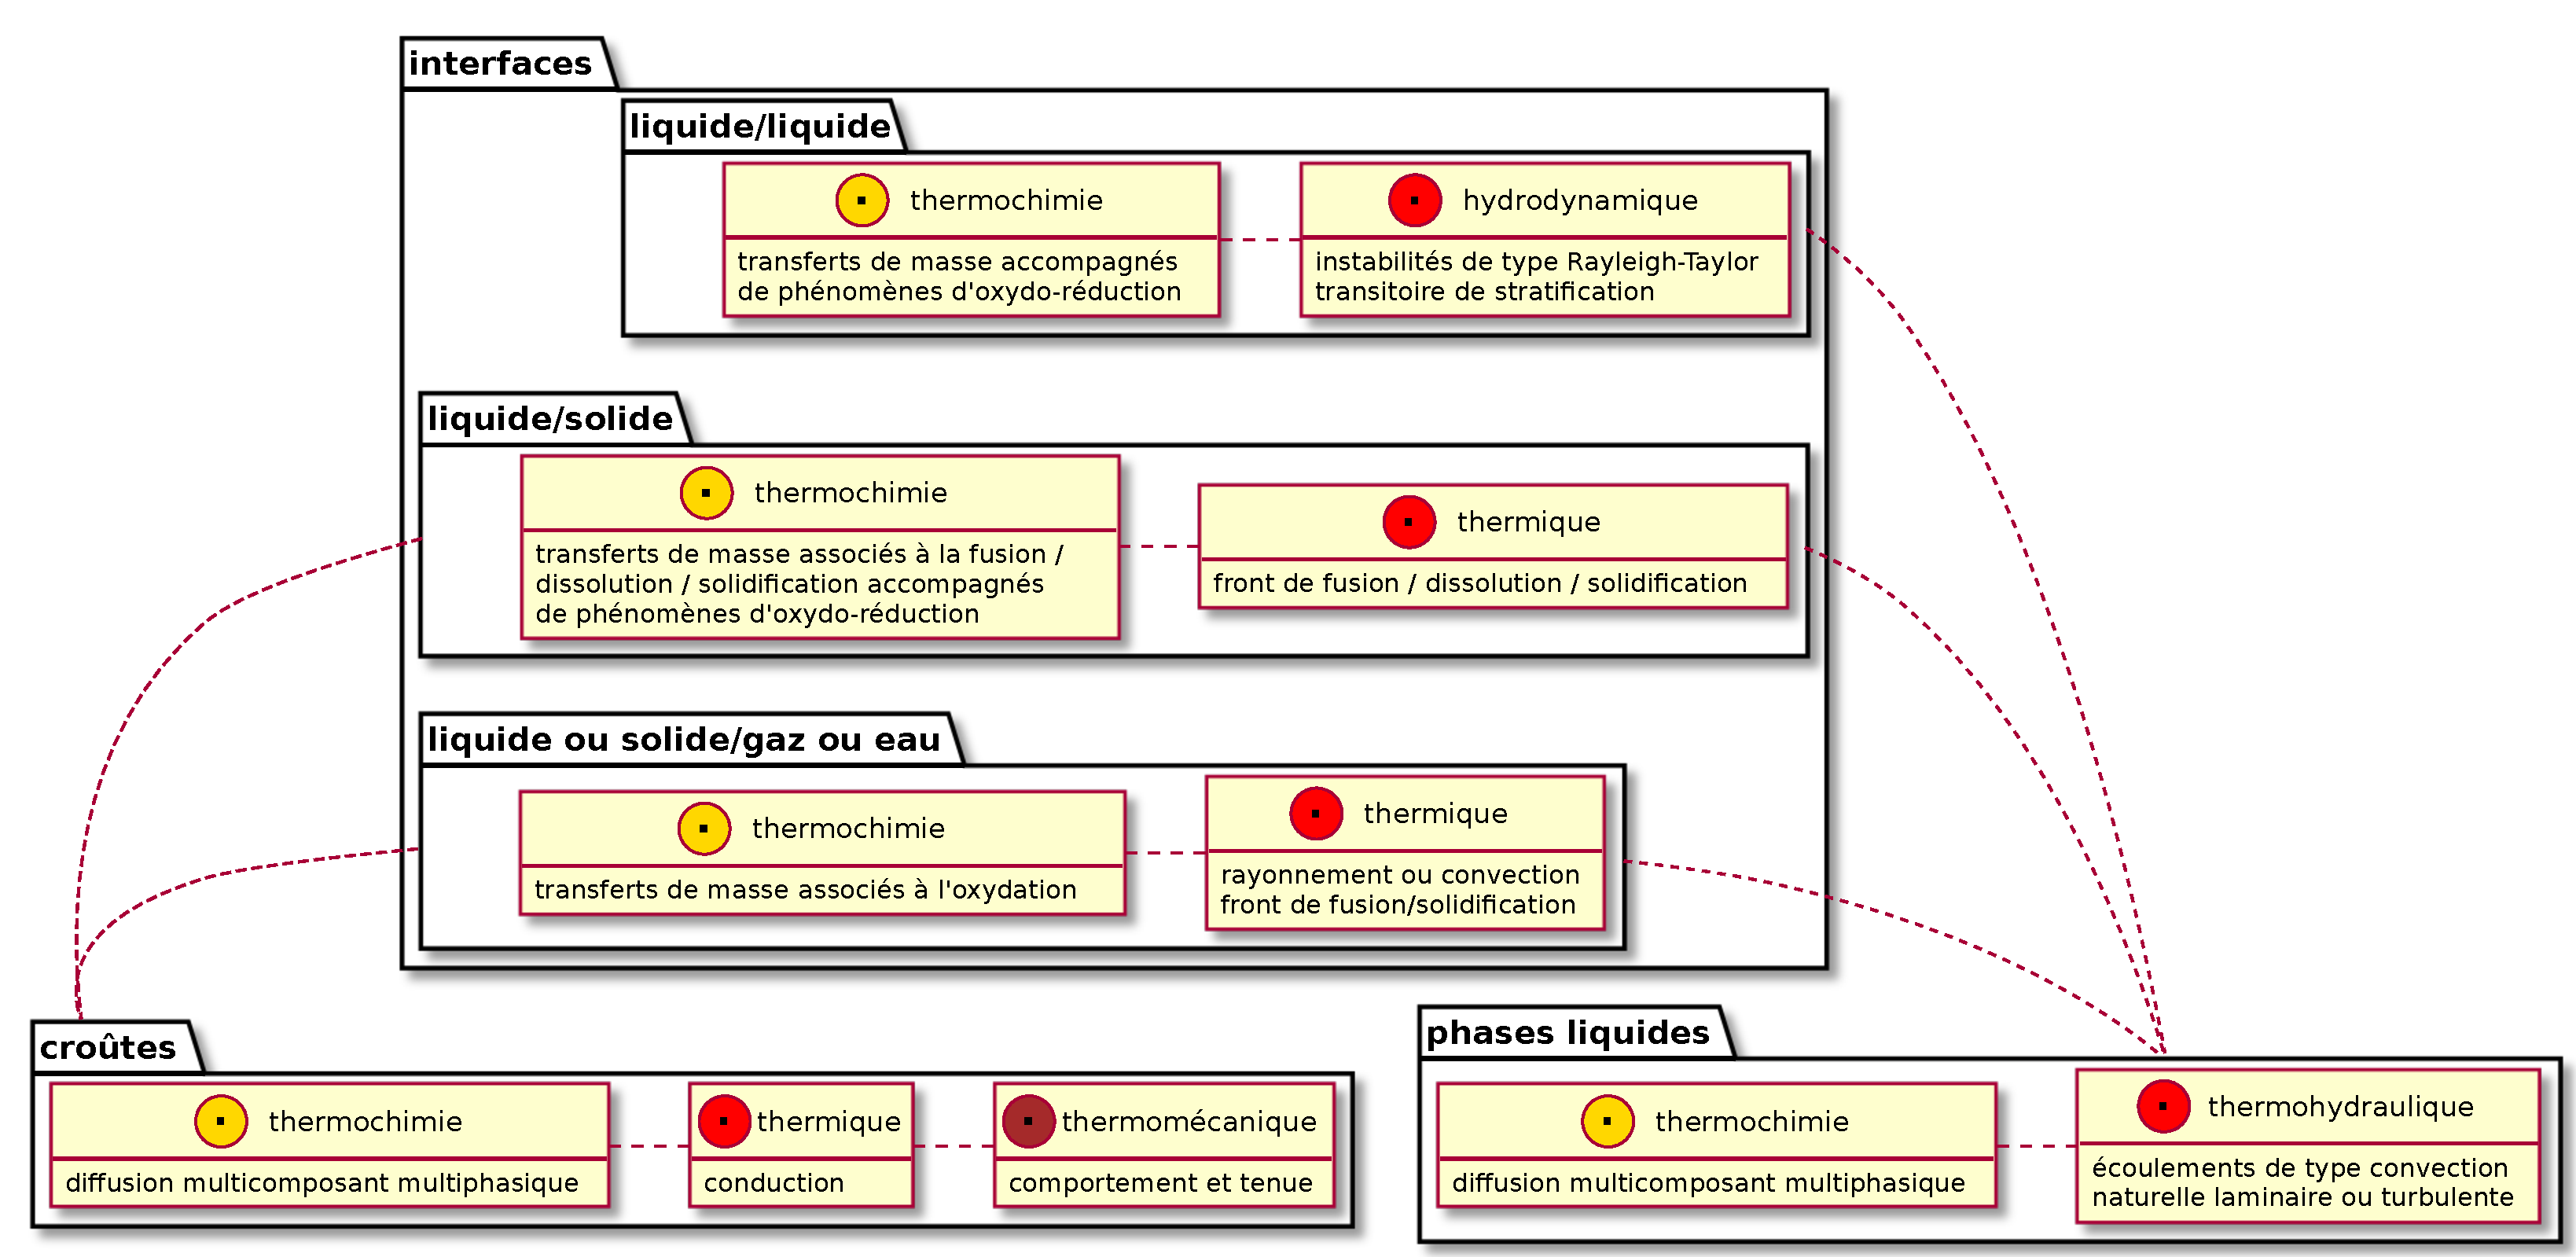
\includegraphics[width=0.7\textwidth]{Figures/corium_en_cuve.pdf}
\vskip -\baselineskip
\caption{\tiny Représentation schématique et partielle de la modélisation du bain de corium en cuve}
\end{figure}
\vskip -0.5\baselineskip
Mais avant de parler de ``thermochimie'', revenons d'abord au \emph{comportement thermohydraulique de la couche mince} et intéressons nous au cas d'une \emph{épaisseur faible} (transitoirement)
\end{itemize}
\end{frame}

%%%%%%%%
\subsection{Thermohydraulique d'une couche métallique supérieure mince}
\begin{frame}[fragile]
\begin{itemize}
\item \emph{Bilan thermique intégral} tel qu'evalué au cours du TD
\begin{columns}[T]
    \begin{column}{0.25\textwidth}
\begin{figure}[H]
\centering 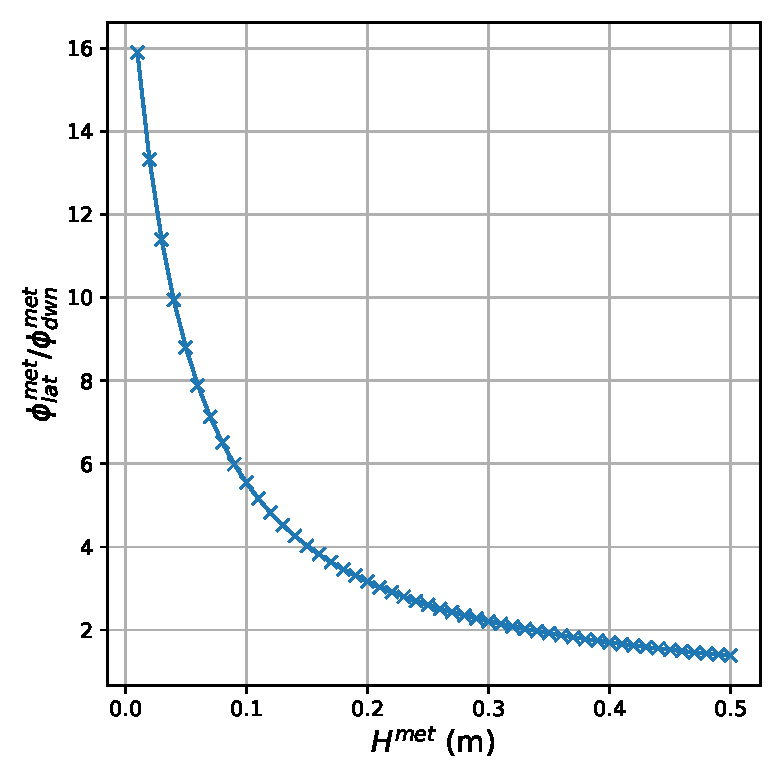
\includegraphics[width=\textwidth]{Figures/Varying_Hmet_2.eps} \\
{\tiny Concentration de flux vs. hauteur de la couche métal (\textit{cf.} TD)}
\end{figure}
    \end{column}
    \begin{column}{0.75\textwidth}
\begin{itemize}
\item Corrélations ``standards'' $\rightarrow$ $\phi^{met}_{lat}/\phi^{met}_{dwn} \nearrow$ lorsque $H^{met} \searrow$ jusqu'à des valeurs très faibles ($<1cm$).
\item Les essais de la campagne BALI-Metal suggère que ces \emph{corrélations surestiment $\phi^{met}_{lat}/\phi^{met}_{dwn}$ pour $H^{met} \le 10$cm}
\item Hormis dans le cas singulier d'une condition adiabatique en surface haute, on s'attend à ce que $\phi^{met}_{lat}/\phi^{met}_{dwn} \rightarrow 0$ quand $H^{met} \rightarrow 0$
\item \emph{Validité de ces corrélations pour cette configuration ?}
\end{itemize}
    \end{column}
\end{columns}
%\item Mais au fait, la surface haute est libre (en l'absence d'oxydation) $\rightarrow$ \emph{quel impact de la déformation de la frontière haute ?}
\item Une question abordée très récemment dans le cadre du projet de recherche européen 
\includegraphics[width=1cm]{Figures/Logo_IVMR.pdf} ~(2015-2019) $\rightarrow$ \emph{illustration de la R\&D menée au CEA}
\end{itemize}
\end{frame}
\subsubsection{Conditions thermiques en limite haute : transfert radiatif et température inhomogène}
\Titre{Couche métallique supérieure - transfert radiatif en surface haute}
\begin{frame}[fragile]
\begin{itemize}
\item Sans le dire, en assimilant le transfert de chaleur vers le haut à celui d'une cavité de Rayleigh-Bénard, on a considéré : \\
\emph{condition inhomogène de transfert radiatif} $\Leftrightarrow$ condition uniforme $T_{up}^{met}$ imposée telle que $\phi_{up}^{BC}\left[T_{up}^{met}\right] = \phi_{up}^{met}\left[T^{met}-T_{up}^{met}\right]$ avec $\phi^{BC}_{up}\left[T^{met}_{up}\right]=\varepsilon_{up}\sigma\left(\left(T^{met}_{up}\right)^4-\left(T^{BC}\right)^4\right)$
\item \emph{Impact de l'inhomogénéité de la condition en limite haute ?}
\item \emph{Etude} paramétrique par \emph{simulations CFD} (code libre 
\includegraphics[width=1cm]{Figures/Logo_TrioCFD.eps} développé au CEA) sur la géometrie parallépipédique des essais BALI-Metal (voir \cite{Peybernes2020})
\begin{itemize}
\item En limite haute, $T_{up}^{met}$ uniforme imposée ou bien condition radiative (locale)
\item $H^{met} \in [1, 10]cm$
\end{itemize}
\begin{columns}[T]
    \begin{column}{0.7\textwidth}
\begin{figure}[H]
\centering 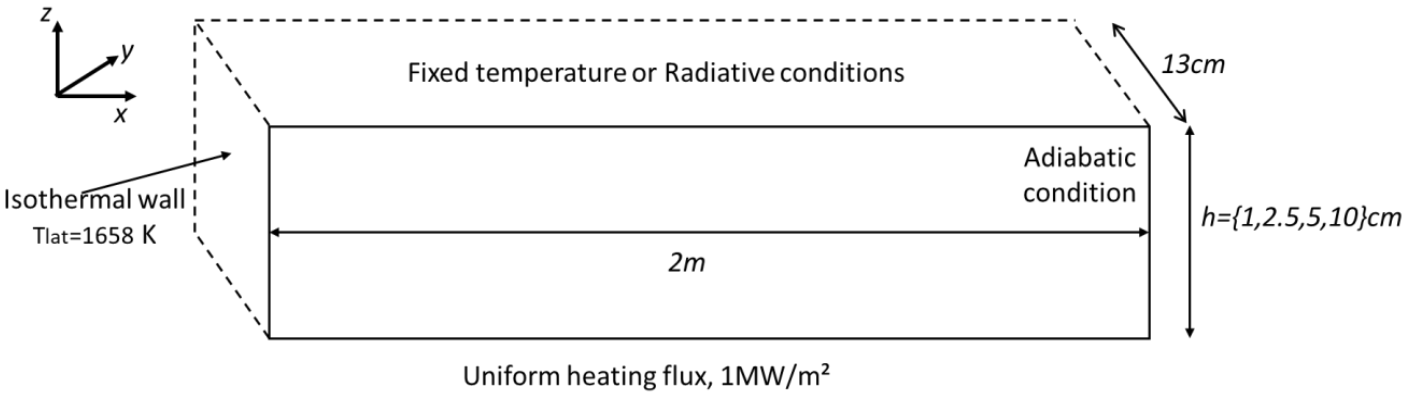
\includegraphics[width=\textwidth]{Figures/Fig3_Peybernes2020.png} \\
{\tiny Domaine de calcul et conditions aux limites des calculs CFD}
\end{figure}
    \end{column}
    \begin{column}{0.3\textwidth}
\begin{figure}[H]
\centering 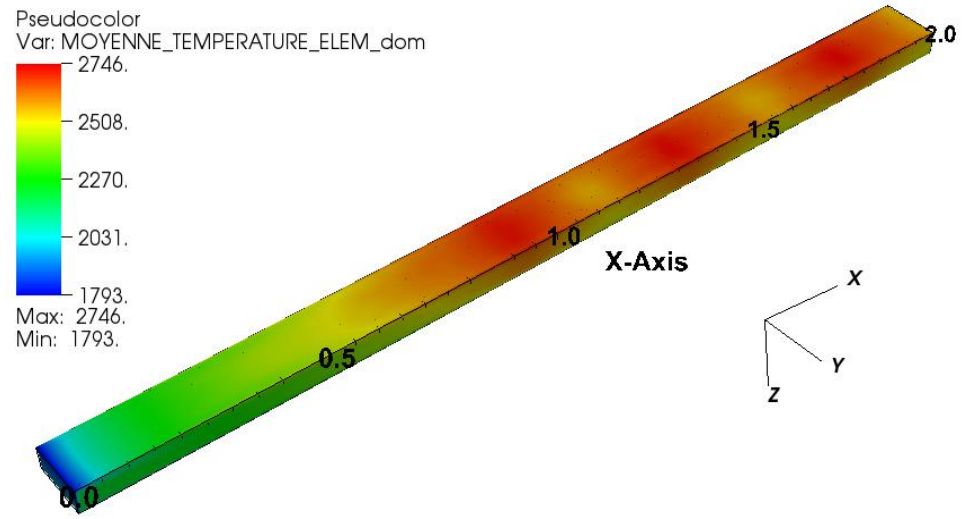
\includegraphics[width=\textwidth]{Figures/Fig5_Peybernes2020.png} \\
{\tiny Température pour $H^{met}=5cm$ (moyennée en temps en régime pseudo-stationnaire)}
\end{figure}
    \end{column}
    \end{columns}
\end{itemize}
\end{frame}
\begin{frame}[fragile]
\vskip -\baselineskip
\begin{columns}[T]
    \begin{column}{0.5\textwidth}
\begin{itemize}
\item \emph{\scriptsize Rôle prédominant de la CL pour $H^{met}$ faible}
\end{itemize}
\vskip -\baselineskip
\begin{figure}[H]
\centering 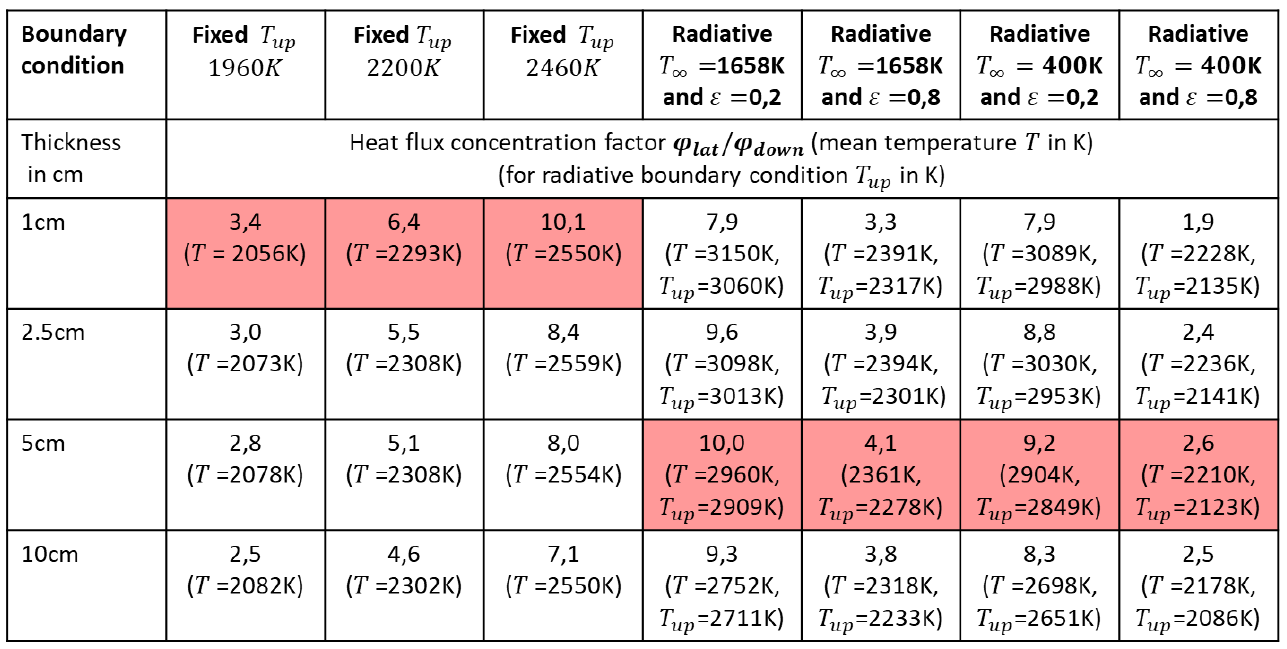
\includegraphics[width=\textwidth]{Figures/TabII_Peybernes2020.png} \\
\vskip -0.5\baselineskip
{\tiny $\phi^{met}_{lat}/\phi^{met}_{dwn}$ fonction de $H^{met}$ et de la condition en limite haute}
\end{figure}
    \end{column}
    \begin{column}{0.5\textwidth}
\vskip -0.8\baselineskip
\begin{figure}[H]
\centering 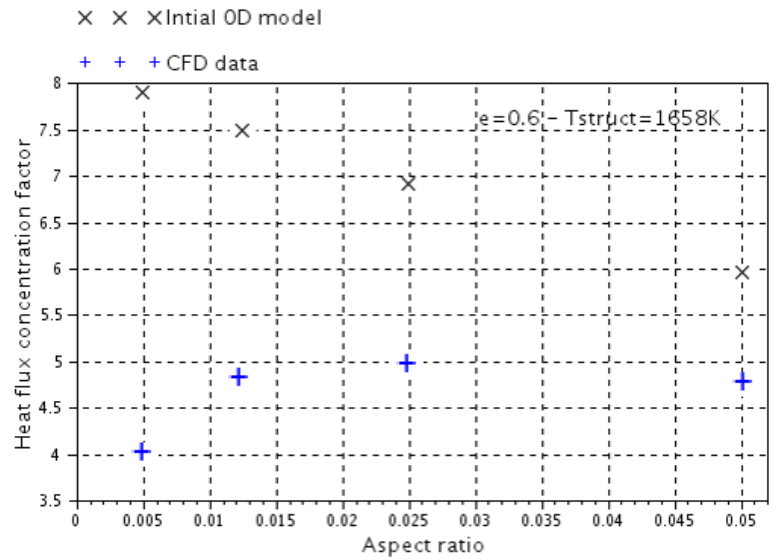
\includegraphics[width=\textwidth]{Figures/Fig6_Peybernes2020.png} \\
\vskip -0.5\baselineskip
{\tiny $\phi^{met}_{lat}/\phi^{met}_{dwn}$ dans le cas $\varepsilon_{up}=0.6$ et $T^{BC}=1658$K}
\end{figure}
    \end{column}
    \end{columns}
\begin{columns}[T]
    \begin{column}{0.6\textwidth}
\begin{figure}[H]
\centering 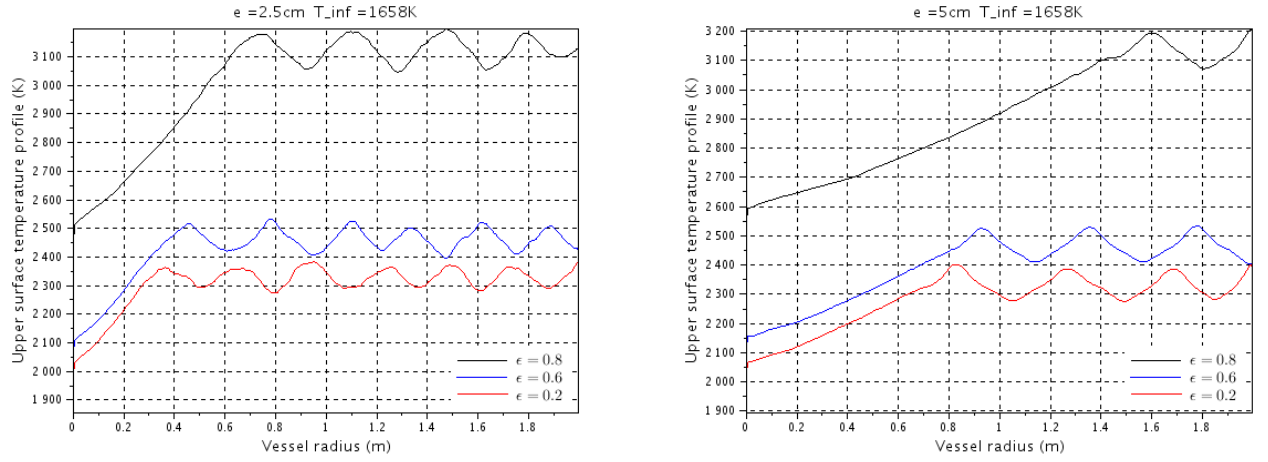
\includegraphics[width=\textwidth]{Figures/Fig8_Peybernes2020.png} \\
\vskip -0.5\baselineskip
{\tiny Profil radiaux de température pour $H^{met}=2.5$cm et $H^{met}=5$cm}
\end{figure}
    \end{column}
    \begin{column}{0.4\textwidth}
\vskip \baselineskip
\begin{itemize}
\item {\scriptsize \emph{Deux nombres adimensionnels} en plus avec \emph{condition radiative}} \\
{\scriptsize e.g. \emph{nombres de Stefan} ($=Pe/Th$) $St \equiv \frac{\varepsilon\sigma T H}{\lambda}$}
\item {\scriptsize Nouvelle corrélation} \\ {\scriptsize $Nu_{up} =  a \times Ra^b Pr^c St_1^d \left(1 + e St_2^f \right)$}
\end{itemize}
    \end{column}
    \end{columns}
\end{frame}
% \subsubsection{Conditions mécaniques en limite haute : Instabilité de Bénard-Marangoni}
% \Titre{Couche métallique supérieure - instabilité de Bénard-Marangoni}
% \begin{frame}[fragile]
% \begin{itemize}
%   \item Frontière supérieure (en l'absence d'oxydation) : une \emph{surface libre déformable}
%   \item Si la \emph{tension de surface $\sigma=f(T)$}, un impact direct sur la thermohydraulique de la couche $\rightarrow$ \emph{effet Marangoni}
%   \item Considérons à nouveau uniquement l'\emph{échange axial} (Rayleigh-Bénard) :
% \begin{columns}[T]
%     \begin{column}{0.35\textwidth}
%     \vskip -\baselineskip
% \begin{figure}[H]
% \centering 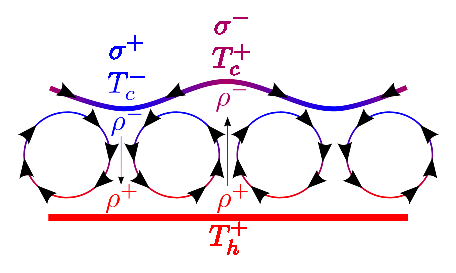
\includegraphics[width=\textwidth]{Figures/RB_BM.eps} \\
%     \vskip -0.5\baselineskip
% {\tiny $\gamma > 0 \rightarrow$ la convection est renforcée}
% \end{figure}
%     \end{column}
%     \begin{column}{0.65\textwidth}
% \begin{itemize}
% \item linéarisation {\scriptsize $\sigma(T) =\sigma_0 - \gamma \left(T-T_0\right)$} avec \emph{$\gamma=-\frac{d\sigma}{dT}(T_0)$}
% \item \emph{$\gamma > 0 \rightarrow$} écoulement de surface dans le \emph{même sens} que cellules de Rayleigh-Bénard
% \item \emph{$\gamma < 0 \rightarrow$} écoulement de surface dans le \emph{sens opposé} des cellules de Rayleigh-Bénard
% \end{itemize}
%     \end{column}
%     \end{columns}
% \item \emph{Instabilité de Bénard-Marangoni} thermique
% \begin{itemize}
% \item $Ma=\frac{\gamma H \Delta T}{\rho_0 \nu \alpha}=\frac{\text{effets thermocapillaires}}{\text{effets dissipatifs (viscosité et diffusion thermique)}}$
% \item \emph{instabilité conditionnelle} (combinée à Rayleigh-Bénard) : \cite{Nield1964} \\
% $\displaystyle \frac{Ra}{Ra_c} + \frac{Ma}{Ma_c} = 1 + \epsilon(Cr,Ga)$ 
% avec $\left\{\begin{array}{rcl} 
%       Cr&=&\frac{\rho\nu\alpha}{\sigma_0 H} ={\tiny\text{déformation de la surface}} \\ 
%       Ga&=&\frac{gH^3}{\nu^2}=\frac{\text{effets de flottabilité}}{\text{effets visqueux}}\end{array}\right.$
% \end{itemize}
% \emph{\textit{a priori}, effet pouvant être important pour $H$ faible}
% \end{itemize}
% \end{frame}
% \begin{frame}[fragile]
% \begin{itemize}
% \item \emph{Evaluation \textit{a priori} pour la couche métallique} (\textit{cf.} \cite{Saas2017})
% \begin{columns}[T]
%     \begin{column}{0.4\textwidth}
%     \vskip -\baselineskip
% \begin{figure}[H]
% \centering 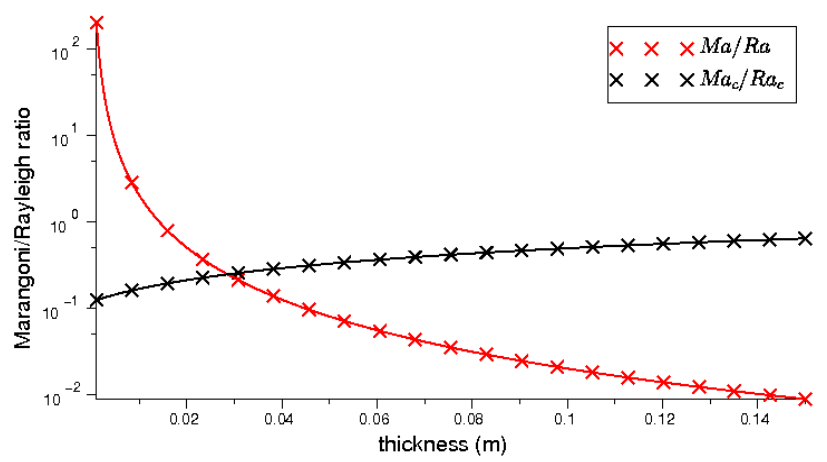
\includegraphics[width=\textwidth]{Figures/Fig3_Saas2017.png} \\
% \end{figure}
%     \end{column}
%     \begin{column}{0.6\textwidth}
%     \vskip -0.5\baselineskip
%     \begin{itemize}
% \item pour $H=0.1$m, en considérant $\Delta T = 100$K et \emph{$\gamma>0$} (fer pur : $4\times 10^{-4}$N.m$^{-1}$.K$^{-1}$), \\
% $Ga\approx 2\times 10^{10}$, $Ra\approx 2\times 10^{7}$, $Ma\approx 5\times 10^{5}$, $Cr\approx 10^{-7}$
% \item \emph{$\frac{Ma}{Ma_c}\ge\frac{Ra}{Ra_c}$ pour $H\le 3$cm}
% \item $Cr\ll 1$ et $Ga\gg 1$: \emph{déformation faible}
% \end{itemize}
%     \end{column}
%     \end{columns}
%     \begin{itemize}
%     \item un effet à prendre en compte \textit{a priori} pour $H \le \sim 5$cm
%     \item simulation simplifée avec une surface plane et une condition limite modifiée : $\cancel{v_x=0} \longrightarrow \frac{\partial v_x}{\partial z} = Ma \frac{\partial T}{\partial x}$
%     \end{itemize}
% \item Mesures de $\sigma(T)$ sur l'installation VITI (CEA Cadarache) \cite{Chikhi2019} : \\ \emph{$\gamma<0$ pour les aciers} 304L (internes cuve) et 16MND5 (paroi cuve)
% \item \emph{Etude} paramétrique par \emph{simulations CFD} (
\includegraphics[width=1cm]{Figures/Logo_TrioCFD.eps}) sur la géometrie parallépipédique des essais BALI-Metal (voir \cite{Peybernes2019})
% \end{itemize}
% \end{frame}
% \begin{frame}[fragile]
% 
% {\footnotesize Quelques résultats extraits de cette étude \cite{Peybernes2019}}
% \begin{columns}[T]
%     \begin{column}{0.6\textwidth}
%     \vskip -\baselineskip
% \begin{figure}[H]
% \centering 
% {\scriptsize $\varepsilon_{up}=0.8$ et $T^{BC}=400$K} \\
% 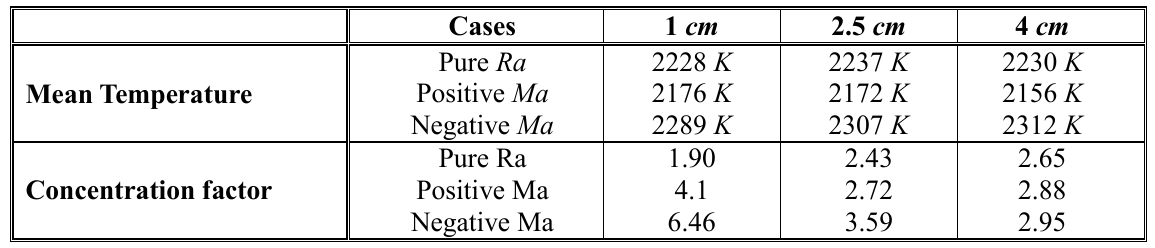
\includegraphics[width=\textwidth]{Figures/TabIV_Peybernes2019.png}
% \end{figure}
%     \end{column}
%     \begin{column}{0.4\textwidth}
%     \begin{itemize}
% \item $T_{(Ra+Ma<0)}>T_{(Ra)}>T_{(Ra+Ma>0)}$
% \item \emph{``Couplage'' fort et non-intuitif avec le refroidissement latéral}
% \end{itemize}
%     \end{column}
%     \end{columns}
% \begin{tabular}{cc}
% \multicolumn{2}{c}{\scriptsize Profil radial de la température de la surface haute ($\varepsilon_{up}=0.2$ et $T^{BC}=1658$K)} \\
% 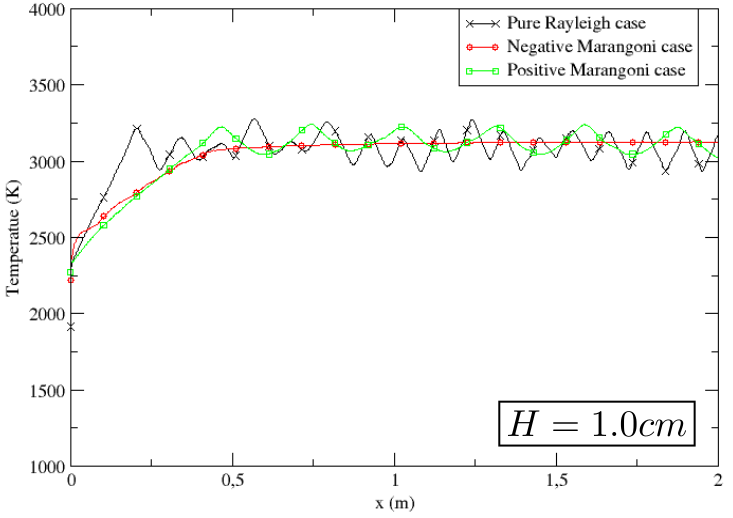
\includegraphics[width=0.35\textwidth]{Figures/Fig5_Peybernes2019.png} & 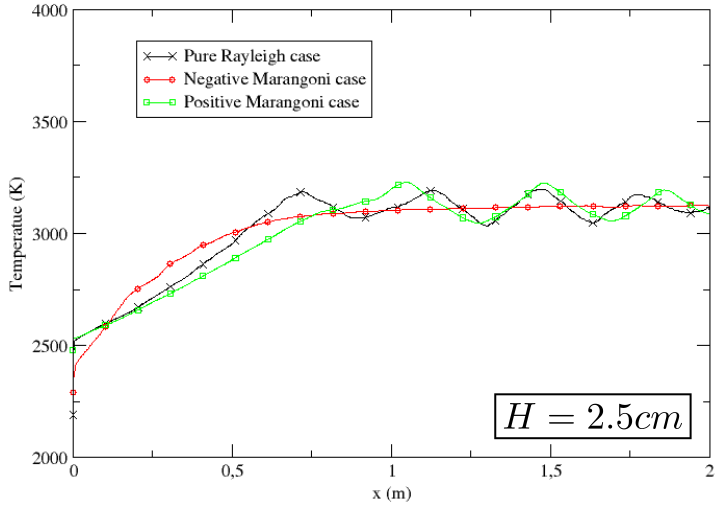
\includegraphics[width=0.35\textwidth]{Figures/Fig6_Peybernes2019.png}
% \end{tabular}
% \begin{itemize}
% \item Loin de la surface latérale, convection ``stoppée'' pour $Ma<0$
% \item Près de la surface latérale, pour $H$ faible, $Ma\lessgtr 0 \rightarrow$ \emph{élargissement de la zone latérale de gradient thermique} $\rightarrow$ refroidissement par transfert radiatif réduit dans cette zone \\
% \emph{Aggravement du focusing effect mais large incertitude} (e.g. $Ma$ solutal, oxydation)
% \end{itemize}
% \end{frame}

%%%%%%%%
\subsection{Corium en cuve et thermochimie}
\Titre{Le corium en fond de cuve: est-ce si simple?}
\begin{frame}[fragile]
Passons maintenant à la \emph{``thermochimie''} {\scriptsize $\left(U_y,Zr_{1-y}\right)O_{2-x}+\left(Fe, \dots\right) \ne$ système ``inerte''}
\begin{figure}[H]
\centering 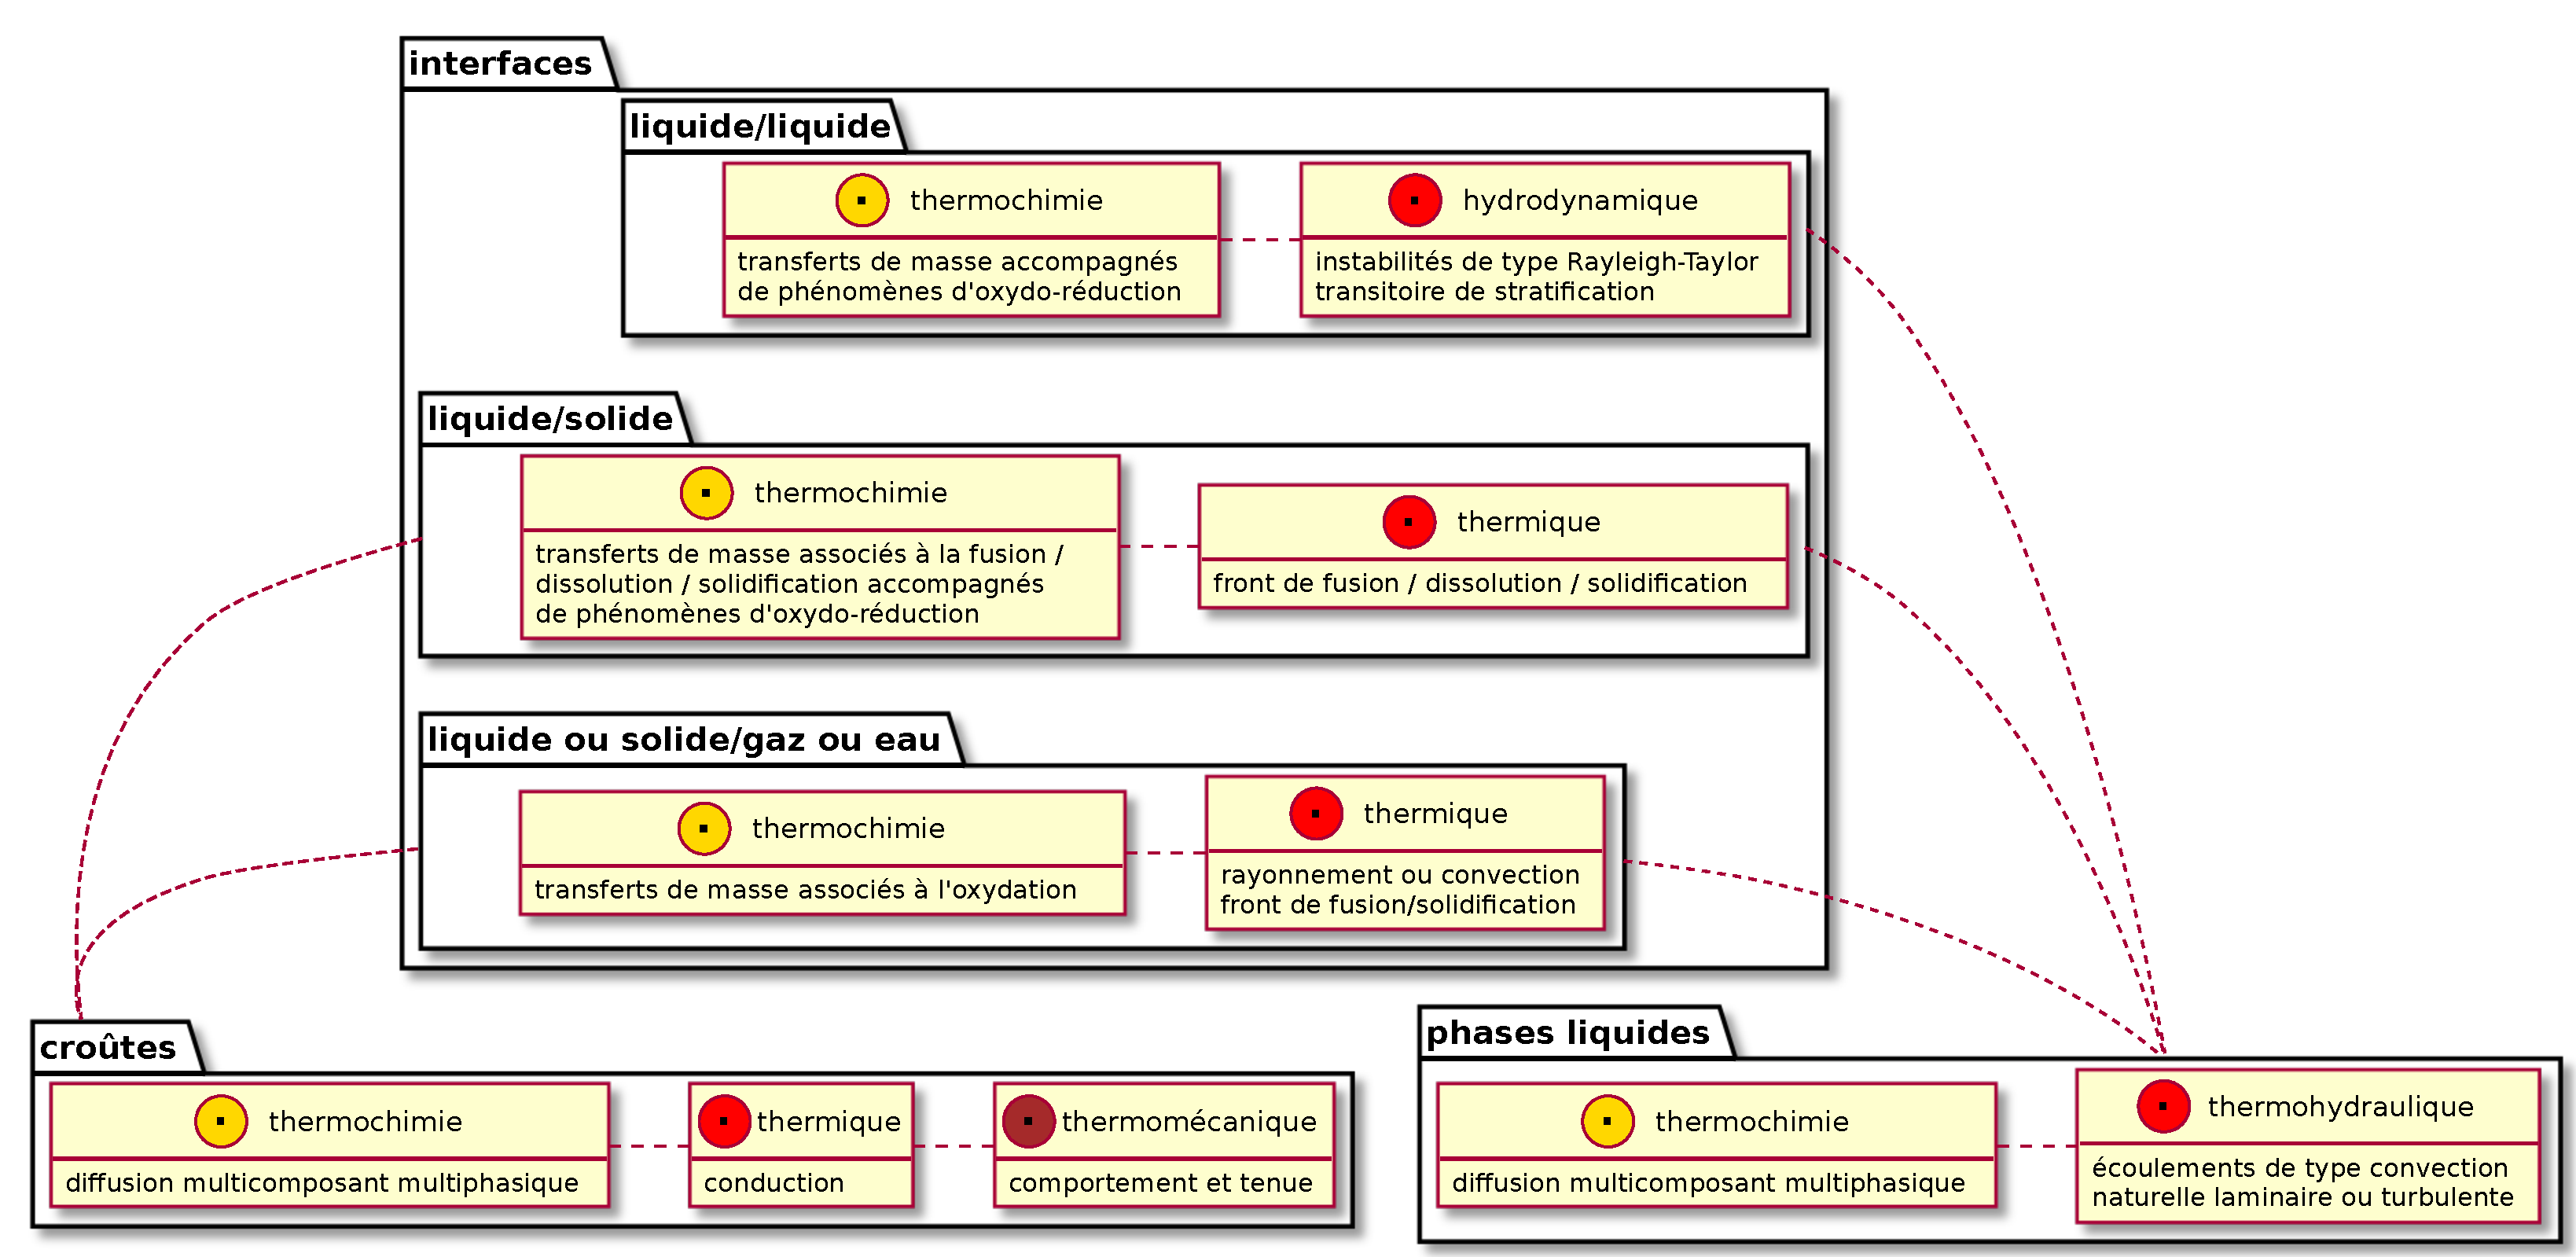
\includegraphics[width=0.75\textwidth]{Figures/corium_en_cuve.pdf}
\vskip -\baselineskip
\caption{\scriptsize Représentation schématique et partielle de la modélisation du bain de corium en cuve}
\end{figure}
\vskip -\baselineskip
\begin{itemize}
\item Nombreux \emph{phénomènes mal connus ou quantifiés}
\item Un phénomène de \emph{premier ordre}, le  \emph{transfert de masse inter-couche} qui, couplé avec l'hydrodynamique, conduit à des \emph{changements de stratification}
\item Présentation de la \emph{phénoménologie} et ouverture sur la \emph{R\&D au CEA} sur ce sujet
\end{itemize}
\end{frame}
\subsection{Stratification des couches liquides}
\Titre{Echanges de masse interfacial et stratification des couches liquides}
\subsubsection{Equilibre thermodynamique de $\left(U_y,Zr_{1-y}\right)O_{2-x}+\left(Fe, \dots\right)$}
\Titre{Equilibre thermodynamique de $\left(U_y,Zr_{1-y}\right)O_{2-x}+\left(Fe, \dots\right)$}
\begin{frame}
      \vskip -0.5\baselineskip
      \begin{itemize}
\item \emph{Lacune de miscibilité} $\rightarrow$ deux liquides à l'\emph{équilibre} ($T$ donnée) avec \emph{$\rho_{met}\lessgtr \rho_{oxy}$} suivant :
\begin{columns}[T]
  \begin{column}{0.45\textwidth}
    \begin{tabularx}{\textwidth}{CCC}
    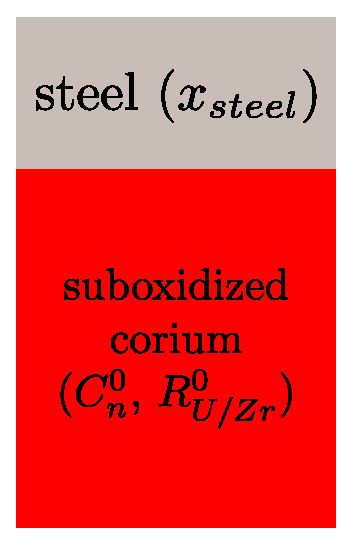
\includegraphics[width=0.2\textwidth]{Figures/schema_stratif_2_ini.eps} & 
    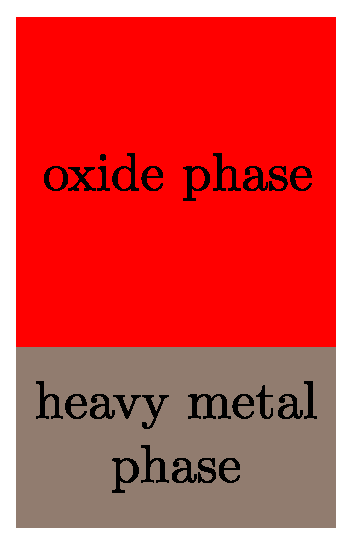
\includegraphics[width=0.2\textwidth]{Figures/schema_stratif_2_hm.eps} &
    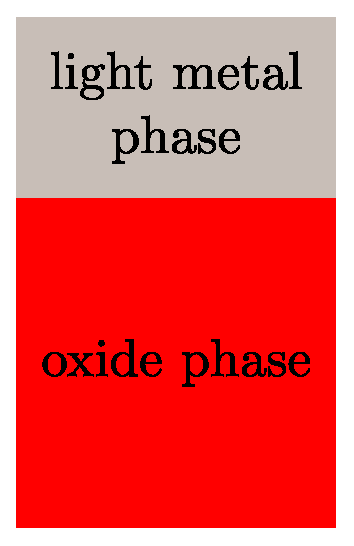
\includegraphics[width=0.2\textwidth]{Figures/schema_stratif_2_lm.eps} \n
    \tiny Etat initial & \tiny Métal ``lourd'' & \tiny Métal ``léger''
    \end{tabularx}
  \end{column}
  \begin{column}{0.6\textwidth} 
  \begin{itemize}
    \item le degré d’oxydation du Zr ($C_n^0$) et du rapport molaire U/Zr ($R_{U/Zr}^0$) du corium oxyde initial
    \item le rapport entre les masses d'acier et de corium oxyde initialement mises en présence ($x_{steel}$)
  \end{itemize}
  \end{column}
\end{columns}
\end{itemize}
\begin{columns}[T]
  \begin{column}{0.4\textwidth}
  \begin{itemize}
    \item \emph{Expériences à ``petite échelle''}
    \item $\diameter \le 7$cm et $m_{oxy}$ $\sim$ 100g à 2kg
    \item e.g. programme MASCA (OCDE) \cite{Tsurikov2007}
  \end{itemize}
  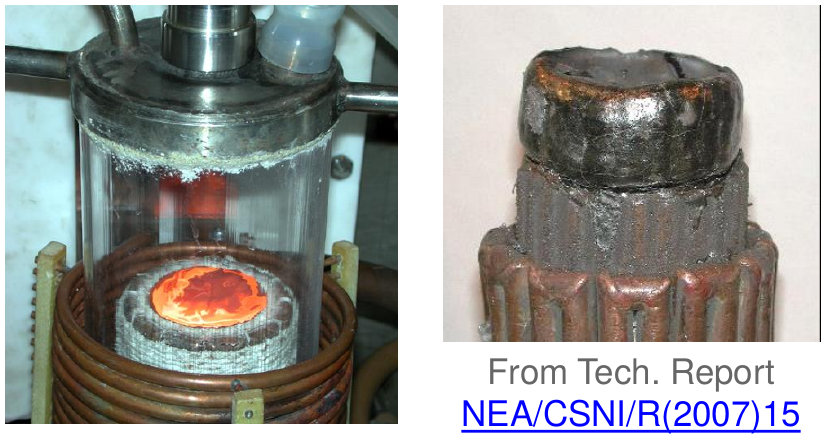
\includegraphics[width=\textwidth]{Figures/rasplav3.png} 
  \end{column}
  \begin{column}{0.6\textwidth} 
\renewcommand{\arraystretch}{0.1}
\centering {\tiny Densités des phases oxyde ($\rho_{oxy}$) et métal ($\rho_{met}$) calculées à l'équilibre}
\begin{tabularx}{\textwidth}{>{\setlength{\baselineskip}{0.5\baselineskip}}C >{\setlength{\baselineskip}{0.5\baselineskip}}C}
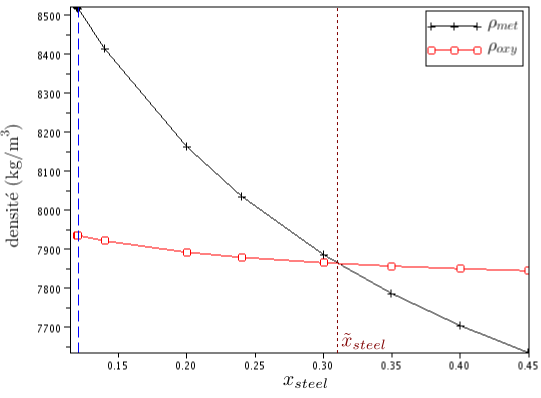
\includegraphics[width=0.48\textwidth]{Figures/densities_vs_x0met_MA3_2840K_new.png} & 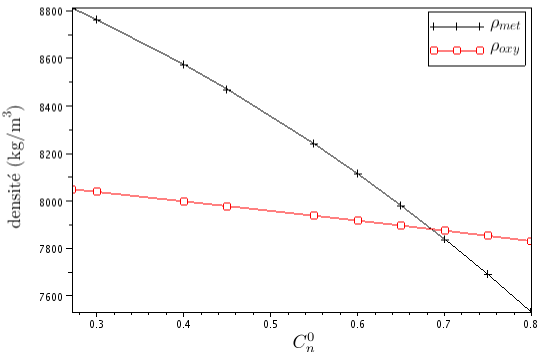
\includegraphics[width=0.48\textwidth]{Figures/densities_vs_Cn_MA9_2855K_new.png} \n
{\tiny En fonction de $x_{steel}$ pour ($\bar{T}=2840$K, $C_n^0=36.5\%$ et $R_{U/Zr}^0=1.14$) $\rightarrow$ MASCA-MA-3} & {\tiny En fonction de $C_n^0$ pour ($\bar{T}=2855$K, $x_{steel}=0.1$ et $R_{U/Zr}^0=1.17$) $\rightarrow$ MASCA-MA-9}
\end{tabularx}
\renewcommand{\arraystretch}{1.0}
      \vskip -0.5\baselineskip
\begin{itemize}
\item Représentation thermodynamique : méthode CALPHAD $\rightarrow$ Energie de Gibbs des phases $\wp$
\item Lois de densité $\rho_{\wp}\left(\text{composition}\right)$
\end{itemize}
  \end{column}
\end{columns}
\end{frame}
\subsubsection{Cinétique de stratification : échange interfacial et instabilité de Rayleigh-Taylor}
\Titre{Cinétique de stratification}
    \begin{frame}
      \vskip -0.5\baselineskip
\begin{columns}[T]
  \begin{column}{0.5\textwidth}
    \begin{tabularx}{\textwidth}{CC}
    \includegraphics[height=0.25\textheight]{Figures/schema_stratif_2_ini.eps} &
    \includegraphics[height=0.30\textheight]{Figures/schema_stratif_3.eps} \n
    \tiny Etat ``initial'' (deux couches) & \tiny Etat transitoire (trois couches)
    \end{tabularx}
  \end{column}
  \begin{column}{0.55\textwidth} 
    \hskip -0.7cm \begin{minipage}{1.1\textwidth}
  \begin{itemize}
\item Transitoire AG en fond de cuve \\ $\rightarrow$ \emph{apport progressif d'acier fondu}
\item \emph{Deux transitoires de stratification} associés à ces équilibres à deux couches potentiels :
\begin{itemize}
\item[\textcolor{OliveGreen}{(1)}] formation de la couche métallique lourde \\
\emph{$\rightarrow$ Aggravement du risque de focusing effect}
\item[\textcolor{blue}{(2)}] retour à une stratification ``normale'' \\
\emph{$\rightarrow$ Remontée de métal ``surchauffé''}
\end{itemize}
  \end{itemize}
\end{minipage}
  \end{column}
\end{columns}
      \begin{itemize}
      \item Ce que l'on peut dire \textit{a priori} des \emph{phénomènes mis en jeu} :
      \begin{itemize}
      \item \emph{transfert de masse interfacial} $\rightarrow$ transitoire \textcolor{OliveGreen}{(1)} : U et Zr vers l’acier \\
      {\tiny (décalage à droite de \ce{ UO_2 + Zr <=> ZrO_2 + U } dans l'oxyde à l’interface)}
      \item transport de masse intra-phase
      \item ``inversion'' de $\rho_{oxy} \lessgtr \rho_{met}$ $\rightarrow$ \emph{instabilité de Rayleigh-Taylor}
      \item mouvement hydrodynamique d'inversion de la position des phases
      \end{itemize}
      \item Deux \emph{cinétiques combinées} : ordres de grandeur pour \textcolor{OliveGreen}{(1)} :
      \begin{itemize}
\item transport de masse intra-phase : $\tau_m = \frac{H^2}{D} \frac{1}{Sh}$ (masse $\Leftrightarrow$ $\tau_h = \frac{H^2}{\alpha} \frac{1}{Nu}$ chaleur) \\
dans le métal, pour $H=5cm$, $Gr\approx4\times 10^{7}$, $Nu\approx10$ (\textit{cf.} TD) \\
en considérant $D=5\times 10^{-9}$m$^2$.s$^{-1}$, $Sh/Nu\approx80$ $\rightarrow$ \emph{$\tau_m \approx 10$min}
\item vitesse terminale de goutte pour l'instabilité de Rayleigh-Taylor $\rightarrow$ \emph{$\sim 10s.m^{-1}$}
      \end{itemize}
      \hskip -0.5cm $\rightarrow$ \emph{Transport intra-phase bien plus lent que mouvement hydrodynamique}
\end{itemize}
    \end{frame}
    \begin{frame}
    
      \emph{\small Observations expérimentales indirectes :}
      \begin{itemize}
      \item Essais à \emph{``petite échelle''} : équilibre atteint en \emph{moins de 20'}, \emph{mouvement ``en bloc''} et très rapide à l'inversion des phases
      \item \emph{Une seule expérience de plus grande échelle} (MASCA-RCW) stoppée au bout de 22' \\ ($\diameter \le 18$cm et $m_{oxy} \approx 45$kg et $x_{steel}\approx 0.1$) - transitoire \textcolor{OliveGreen}{(1)}
      \begin{columns}
\begin{column}{0.65\textwidth}
\vskip 0.5\baselineskip
\includegraphics[width=\textwidth]{Figures/rcw.png}
\end{column}
\begin{column}{0.4\textwidth}
\hskip -0.8cm \begin{minipage}{1.1\textwidth}
  \begin{itemize}
\item état final $\sim$ un instant du transitoire de formation de la phase métallique lourde
\item Rayleigh-Taylor en gouttelettes
\item gradient de concentration en U, Zr dans la couche métallique supérieure
\end{itemize}
\end{minipage}
\end{column}
      \end{columns}
      \item \emph{Cinétique limitante : celle du transfert de masse} (transport multicomposant, multiphasique)
      \item Pour les cas réacteurs, évaluation du temps caractéristique : \\ $\sim 1$h pour \textcolor{OliveGreen}{(1)} et plus élevé pour \textcolor{blue}{(2)} ...
\end{itemize}
    \end{frame}
\begin{frame}[fragile]
\begin{itemize}
\item ... Une \emph{incertitude forte} / des modèles (intégraux) en manque de calage/validation
\begin{itemize}
\item MASCA-RCW ne donne qu'un information indirecte sur le transitoire
\item Aucune expérience caractérisant le transitoire \textcolor{blue}{(2)} de retour à une stratification ``normale'' 
\item Impact d'une croûte à l'interface oxyde/acier
\end{itemize}
\item \emph{Important ! $\rightarrow$ meilleure quantification du comportement transitoire du corium en cuve}
\item En particulier, \emph{R\&D au CEA} :
\begin{columns}
 \begin{column}{0.55\textwidth}
\begin{itemize}
\item Modélisation et \emph{simulation ``mésoscopique''} (CFD) \cite{Zanella2020}
\item Caractérisation expérimentale de la \emph{dissolution d'une croûte de corium oxyde par de l'acier fondu} \cite{Pivano2019}
\item Conception d'un \emph{dispositif experimental \\ $\sim$ MASCA-RCW} mais avec \emph{suivi en ligne des interfaces} par mesure acoustique \cite{Cavaro2019}
\end{itemize}
 \end{column}
 \begin{column}{0.1\textwidth}
 \begin{minipage}{\textwidth}
\movie[showcontrols,width=\textwidth,height=0.5\textheight,externalviewer]{\includegraphics[height=0.5\textheight]{Figures/movie_RT_snapshot.eps}}{Figures/movie_RT.mov}
\end{minipage}
 \end{column}
 \begin{column}{0.35\textwidth}
 \includegraphics[width=\textwidth]{Figures/cormet.png} \\
 \includegraphics[width=\textwidth]{Figures/stromboli.png}
 \end{column}
\end{columns}
\end{itemize}
\end{frame}
\Intercalaire{Illustration du risque de percement de la cuve en transitoire \\ Résultats de simulation avec le code PROCOR \\ (développé au CEA Cadarache)}
\section{Illustration du risque de percement de la cuve en transitoire}
\Titre{Illustration du risque de percement de la cuve en transitoire : résultats PROCOR}
\begin{frame}[fragile]
\vskip -0.8\baselineskip
\begin{figure}[H]
\centering \includegraphics[height=\textheight]{Figures/procor_0a.pdf} 
\end{figure}
\end{frame}
\begin{frame}[fragile]
\vskip -0.8\baselineskip
\begin{figure}[H]
\centering \includegraphics[height=\textheight]{Figures/procor_0b.pdf} 
\end{figure}
\end{frame}
\begin{frame}[fragile]
\vskip -0.8\baselineskip
\begin{figure}[H]
\centering \includegraphics[height=\textheight]{Figures/procor_1.pdf} 
\end{figure}
\end{frame}
\begin{frame}[fragile]
\vskip -0.8\baselineskip
\begin{figure}[H]
\centering \includegraphics[height=\textheight]{Figures/procor_2.pdf} 
\end{figure}
\end{frame}

%%%%%%%%
\Intercalaire{Introduction au code PROCOR}
\section{Introduction au code PROCOR}
\Titre{Introduction au code PROCOR}
\begin{frame}[fragile]
\end{frame}

%%%%%%%%%%%%%%%%%%%%%%%%%%%%%%%%%%%%%%%%%%%%%%%%%%%%%%%%%%%%%%%%%%%%%%%%%%%%%%%%%%%%%%%%%%%%%%%%%%%%%%%%%%%%%%%%%%%%%%%%%%%%%%%%%%%%%%%%%%%%%%%%%%%%%%%%%

%%%%%%%%
\Intercalaire{Introduction au calcul statistique avec PROCOR/URANIE}
\section{Introduction au calcul statistique avec PROCOR/URANIE}
\Titre{Introduction au calcul statistique avec PROCOR/URANIE}
\begin{frame}[fragile]
Pourquoi des calculs statistiques ?
\begin{itemize}
\item Gérer la méconnaissance de paramètres ou de données d'entrée au système à résoudre.
\item Participer à l'amélioration de la connaissance de la phénoménologie (cf. transparent "La démarche phénoménologique dans PROCOR").
\end{itemize}

3 catégories d’incertitudes :

\begin{itemize}
\item Aléatoires (e.g. précision du système de mesure, fluctuation de l’environnement…) et
incompressibles
\begin{itemize}
\item densité de probabilité (pdf)
\end{itemize}
\item Épistémiques (manque de connaissance)
\begin{itemize}
\item \textit{a priori} pas de pdf
\item Expertise : plage de variation
\item Une pdf peut-être supposée (degré de croyance)
\end{itemize}
\item Mixtes (aléatoire et épistémiques)
\end{itemize}



\end{frame}



\Titre{Introduction au calcul statistique avec PROCOR/URANIE}
\begin{frame}[fragile]

Approche probabiliste des incertitudes dans la simulation :
\begin{itemize}
\item Grandeurs incertaines \(\rightarrow\) Variables aléatoires
\begin{itemize}
\item Incertitudes = densité de probabilité (pdf) de la variable aléatoire
\end{itemize}
\end{itemize}

Processus typique des études statistiques :


\begin{figure}
\centering \includegraphics[width=0.75\textwidth]{Figures/Stat_1.png} 
\end{figure}


\end{frame}


\Titre{Introduction au calcul statistique avec PROCOR/URANIE}
\begin{frame}[fragile]
Qu'entend-on par "études statistiques" ?
\begin{itemize}
\item Etudes paramétriques
\begin{itemize}
\item Définition d’une plage de variation d’Entrées
\(\rightarrow\) plage de variation des Sorties
(palliatif au manque de connaissance des Entrées)
\end{itemize}
\item Analyse de sensibilité (incertitudes avec pdf )

\begin{itemize}
\item A partir des incertitudes des Entrées
\(\rightarrow\) quantifier la sensibilité du système à chaque Entrée
(classement des Entrées par degré d’influence)
\end{itemize}

\item Propagation d’incertitudes
\begin{itemize}
\item A partir des incertitudes (exhaustives et précises) des Entrées
\(\rightarrow\) Incertitudes des Sorties
(précision du calcul)
\end{itemize}

\end{itemize}

\end{frame}




\Titre{Introduction au calcul statistique avec PROCOR/URANIE}
\begin{frame}[fragile]
Sources d'incertitudes pour les Accidents Graves
\begin{figure}
\centering \includegraphics[width=0.95\textwidth]{Figures/Stat_OriginesIncert.png} 
\end{figure}


\end{frame}


\Titre{Introduction au calcul statistique avec PROCOR/URANIE}
\begin{frame}[fragile]
En pratique, un \emph{outil spécifique pour PROCOR} (\textit{statistics}) a été construit sur la base de la plateforme URANIE.\\
\emph{URANIE} est la plateforme du CEA pour la propagation d'incertitudes, elle-même basée sur l'outil \emph{ROOT} du CERN.
Cela permet une utilisation facilité des fonctionnalités d'URANIE. Les grandes étapes sont: 
\begin{itemize}
\item définition des paramètres d'entrée à probabiliser \\
dans un fichier \textit{template} du même type que \texttt{ap1000\_benchmark\_parameter\_input\_file.txt} , en remplaçant la valeur du paramètre par \textit{xxx}

\item définition des loi statistiques suivies par les pdf de ces paramètres et du nombre de calculs à réaliser\\
dans un fichier spécifique \texttt{input.uranie}

\item définition des paramètres de sortie qui seront observés \\
dans un fichier \texttt{output.uranie} permettant de renommer les sorties avec des alias et de leur donner une valeur par défaut.

\end{itemize}

\end{frame}


\Titre{Introduction au calcul statistique avec PROCOR/URANIE}
\begin{frame}[fragile]


Processus du calcul statistique : 
\begin{itemize}
    \item échantillonnage (tirage aléatoire) des valeurs des paramètres d'entrée compte tenu de leur loi de pdf et du nombre de calcul à effectuer
    \item création des fichiers d'entrée \texttt{ap1000\_benchmark\_parameter\_input\_file.txt} pour chaque calcul
    \item lancement des calculs
    \item récupération des valeurs des sorties observées dans un tableau comprenant les valeurs des entrées et des sorties
\end{itemize}



\end{frame}


\Titre{Introduction au calcul statistique avec PROCOR/URANIE}
\begin{frame}[fragile]
L'outil \textit{statistics} calcule deux grandeurs :
\begin{itemize}
    \item la probabilité d'un évènement (variable aléatoire \textit{X}, entre 0 et 1)
\end{itemize}
\begin{figure}
\centering \includegraphics[width=0.95\textwidth]{Figures/Stat_EventProba.png} 
\end{figure}

\begin{itemize}
    \item le ratio de corrélation d'un paramètre \textit{P} étant donné un évènement \textit{X}
\end{itemize}
\begin{figure}
\centering \includegraphics[width=0.95\textwidth]{Figures/Stat_CorrelationRatio.png} 
\end{figure}



\end{frame}


\Titre{Introduction au calcul statistique avec PROCOR/URANIE}
\begin{frame}[fragile]
Le post-traitement avec ROOT est à la charge de l'utilisateur. Cf. page du wiki PROCOR pour l'utilisation de ROOT pour PROCOR (fournie séparément).


\begin{itemize}
    \item Mise en pratique sur le cas n$^{\circ}$3. Pour des raisons de temps de calculs, les calculs ont déjà été réalisés avec un choix des paramètres d'entrée probabilisés : 
    
    \begin{itemize}
        \item A définir
    \end{itemize}
\end{itemize}

    \item Objectif : identifier les paramètres d'entrée influents et choisir la meilleur représentation pour illustrer ce choix.



\end{frame}


%%%%%%%%%%%%%%%%%%%%%%%%%%%%%%%%%%%%%%%%%%%%%%%%%%%%%%%%%%%%%%%%%%%%%%%%%%%%%%%%%%%%%%%%%%%%%%%%%%%%%%%%%%%%%%%%%%%%%%%%%%%%%%%%%%%%%%%%%%%%%%%%%%%%%%%%%
\DernierePage{}
\Annexes
\section*{Références}
\Titre{Références}
\begin{frame}[fragile,allowframebreaks]
  \bibliography{lma-jabref}
\end{frame}
%%
\end{document}
%% definition du dictionnaire local
<!-- Local IspellDict: francais -->
